\documentclass[a4paper,12pt, twoside]{book}
\usepackage{lmodern}
\newlength\longest
\usepackage{scrextend}
\usepackage{graphicx}
\usepackage[utf8]{inputenc}
\usepackage[T1]{fontenc} 
\usepackage{fouriernc}
\usepackage[document]{ragged2e}
\usepackage{amsmath}
\usepackage{amssymb}
\graphicspath{ {images/} }
\usepackage{hyperref}
\usepackage{macros}
\usepackage[normalem]{ulem}
\usepackage[]{algorithm2e}
\usepackage{pgf,tikz}
\usepackage{pgfplots}
\usepackage[signature=default_signature, date=01.06.2019]{mysignature}
\usetikzlibrary{spy}
\usetikzlibrary{backgrounds}
\usetikzlibrary{decorations.pathreplacing}
\usetikzlibrary{intersections}
\usepackage[margin=0.8in, right= 0.6in]{geometry}
\usepackage{textcomp}
\usetikzlibrary {automata,positioning}
%\usepackage {xcolor}
\definecolor {processblue}{cmyk}{0.96,0,0,0}
\usepackage{fancyhdr}
\pagestyle{fancy}
\fancyhead{}
\fancyhead[RO,LE]{Reachability Games with strong and relaxed energy constraints}
\fancyfoot{}
\fancyfoot[LE,RO]{\thepage}
\fancyfoot[LO,CE]{Chapter \thechapter}
\fancyfoot[CO,RE]{Ritam Raha}
\usepackage[nottoc,numbib]{tocbibind}
\usepackage{amsthm}
\theoremstyle{definition}
\newtheorem{theorem}{Theorem}[section]
\newtheorem{claim}[theorem]{Claim}
\newtheorem{conjecture}[theorem]{Conjecture}
\newtheorem{corollary}[theorem]{Corollary}
\newtheorem{definition}[theorem]{Definition}
\newtheorem{example}[theorem]{Example}
\newtheorem{fact}[theorem]{Fact}
\newtheorem{lemma}[theorem]{Lemma}
\newtheorem{proposition}[theorem]{Proposition}
\newtheorem{remark}[theorem]{Remark}

\begin{document}
\begin{titlepage}
	\centering
	\scshape 
	{\LARGE{CHENNAI MATHEMATICAL INSTITUTE}}\\
          \vskip 0.5cm
	MASTERS THESIS
	\vspace*{\baselineskip} 
	%------------------------------------------------
	%	Title
	%------------------------------------------------
	
	\rule{\textwidth}{1.6pt}\vspace*{-\baselineskip}\vspace*{2pt}
	\rule{\textwidth}{0.4pt} 

	\vspace{0.75\baselineskip}
	
	{\LARGE REACHABILITY GAMES WITH\\ strong and relaxed \\ ENERGY CONSTRAINTS\\} 
	
	\vspace{0.75\baselineskip} 
	
	\rule{\textwidth}{0.4pt}\vspace*{-\baselineskip}\vspace{3.2pt} 
	\rule{\textwidth}{1.6pt}
	
	\vspace{2\baselineskip} 
	
	%------------------------------------------------
	%	Author
	%------------------------------------------------
	
	
	
	\textit{Author:}
	
	\vspace{0.5\baselineskip} 
	
	{\scshape\Large Ritam Raha}\\ % Author
	\vspace{0.2\baselineskip}
	{\small Chennai Mathematical Institute}
	\vspace{2\baselineskip} 

		
	\textit{Supervised by:}     
	\vspace{0.5\baselineskip}

	{\scshape\Large Nicolas Markey}\ \ \ \ \&\ \ \ \  {\scshape\Large Loïc Hélouët}\\ % Supervisors
	\vspace{0.2\baselineskip}
	{\small INRIA Rennes}
	\vspace{2\baselineskip}

	\vspace{2\baselineskip} 
	
	\textit{A thesis submitted in fulfillment of the requirements\\ for the degree of Master of Science}\\
	\vspace{1\baselineskip}
	\textit{in the}\\
	\vspace{1\baselineskip}
	{\scshape Department of Computer Science\\ Chennai Mathematical Institute}

	\vspace{4\baselineskip}
	
	
\includegraphics[width=0.7\textwidth]{cmi.png}

	\vfill % Whitespace between editor names and publisher logo
	
\end{titlepage}

\chapter*{Declaration}
I, Ritam RAHA, declare that this thesis titled, \textit{“Reachability Games with strong and relaxed energy constraints”} and the work presented in it are my own. I confirm that:
\vskip 1cm
\begin{itemize}
    \item This work was done wholly or mainly while in candidature for a masters degree(from CMI) at INRIA Rennes and CMI.
    \item The thesis has been prepared without resorting to plagiarism.
    \item Where I have consulted the published work of others, this is always clearly attributed.
    \item I have acknowledged all main sources of help.
    \item The thesis has not been submitted elsewhere for a degree.
\end{itemize}
\vskip 2cm
\mysignature[left]{full}

\chapter*{
%Quotes
}

\thispagestyle{empty}
\null\vfill

\settowidth\longest{\huge\itshape just as his inclination leads him;}
\begin{center}
\parbox{\longest}{%
  \raggedright{\huge\itshape%
   "The problem is \\ 
  not the problem; \\
  The problem is your attitude \\ 
  about the problem."\par\bigskip
  }   
  \raggedleft\Large\MakeUppercase{- Jack Sparrow}, \textit{Pirates of the Caribbean}\par%
}
\end{center}

\vfill\vfill

\chapter*{Abstract}
Quantitative reachability games are finite two player turn-based games played on weighted graphs. The objective of the game combines reachability objective(qualitative) with the (quantitative) requirement that the weights along a path must satisfy certain constraints (bounds). Besides having direct applications in reactive system synthesis with resource constraints, it is one of the simplest models that combine quantitative and qualitative objectives.
\vskip 0.5cm
In this thesis, we~first prove that under strict energy constraints (either only
lower-bound constraint or interval constraint), those games are
LOGSPACE-equivalent to energy games with the same energy constraints but without reachability objective (i.e., for infinite
runs). We~then consider two kinds of
relaxations of the upper-bound constraints (while keeping the
lower-bound constraint strict): in the first one, called \emph{weak
upper bound}, the upper bound is \emph{absorbing}, in the sense that
it allows receiving more energy when the upper bound is already
reached, but the extra energy will not be stored; in the second one,
we~allow for \emph{temporary violations} of the upper bound, imposing
limits on the number or on the amount of violations.

%
We prove that when considering weak upper bound, reachability
objectives require memory, but can still be solved in polynomial-time
for one-player arenas; we~prove that they are in coNP in the two-player
setting. Allowing for bounded violations makes the
problem PSPACE-complete for one-player arenas and EXPTIME-complete
for two players.

\chapter*{%Dedication}
}
I dedicate this to 
 


\chapter*{Acknowledgements}
I want to thank...

\tableofcontents

\chapter{Introduction}
\paragraph{Games on weighted graphs.}
Weighted games are a common way to formally address questions
related to consumption, production and storage of resources: the arena
of such game are two-player turn-based games in which transitions
carry positive or negative integers, representing the accumulation or
consumption of resource.  Various objectives have been considered for
such arenas, such as optimizing the total or average amount of
resources that have been collected along the play, or maintaining the
total amount within given bounds. The~latter kind of objectives,
usually referred to as \emph{energy
objectives}~\cite{CdAHS03,BouyerFLMS08}, has been widely studied in
the untimed
setting~\cite{ChatterjeeD12,ChatterjeeDHR10,DDGRT10,FahrenbergJLS11,JLR13,
JLS15,VCDHRR15,BMRLL15,BHMRZ17,DM18}, and to a lesser extent in the
timed setting~\cite{BFLM10,qest2012-BLM}.
%
As their name indicates, energy objectives can be used to model the
evolution of the available energy in an autonomous system: besides
achieving its tasks, the~system has to take care of recharging
batteries regularly enough so as to never run out of power.  Energy
objectives were also used to model moulding machines: such machines
inject molten plastic into a mould, using pressure obtained by storing
liquid in a tank~\cite{CJLRR09}; the~level of liquid has to be
controlled in such a way that enough pressure is always available, but
excessive pressure in the tank would reduce the service life of the valve.

Energy games impose strict constraints on the total amount of energy
at all stages of the play. Two kinds of constraints have been mainly
considered in the literature: lower-bound constraints (a.k.a. L-energy constraints) impose a strict lower bound (usually~zero), but impose no
upper bound; on~the other hand, lower- and upper-bound constraints
(a.k.a. LU-energy constraints) require that the energy level always
remain within a bounded interval~$[L;U]$. Finding strategies that
realize L-energy objectives along infinite runs is in PTIME in the
one-player setting, and in NP $\cap$ coNP for two players;
for LU-energy objectives, it~is respectively PSPACE-complete
and EXPTIME-complete~\cite{BouyerFLMS08}. Some works have also considered
the existence of an initial energy level for which a winning strategy
exist~\cite{ChatterjeeDHR10}.
%
Energy objectives have also been combined with other objectives,
either qualitative (e.g.~parity~\cite{ChatterjeeD12}) or quantitative
objectives (e.g.~multi-dimensional
energy~\cite{ChatterjeeDHR10,FahrenbergJLS11,JLR13}). 

In this paper, we focus on weighted games combining energy objectives
together with reachability objectives. Our~first result is the
(expected) proof that L-energy games with or without reachability
objectives are interreducible; the same holds for LU-energy games.

%
We~then focus on relaxations of the energy constraints, in two
different directions. In both cases, the lower bound remains
unchanged, as it corresponds to running out of energy, which we always
want to avoid. We~thus only relax the upper-bound constraint.
The~first direction concerns \emph{weak upper bounds}, already
introduced in~\cite{BouyerFLMS08}: in~that setting, hitting the upper bound
is allowed, but there is no overload, i.e. trying to exceed the upper bound will simply maintain the energy level at this maximal level. Yet, a strict lower bound is
still imposed. We~name these objectives LW-energy
objectives. This~could be used as a (simplified) model for batteries.
When considered alone, LW-energy objectives are not much different
from~ L-energy objectives, in the sense that the aim is to find a
reachable \emph{positive loop}. LW-energy games are in PTIME for
one-player games, and in NP $\cap$ coNP for two players. When
combining LW-energy and reachability objectives, the~situation
changes: different loops may have different effects on the energy
level, and we have to keep track of the final energy level reached
when iterating those loops.

The second way of relaxing upper bounds, which we call \emph{soft
upper bound}, allows a limited number (or amount) of
violations: when modeling a pressure tank, the lower-bound constraint
is strict (pressure should always be available) but the upper bound is
soft (excessive pressure may be temporarily allowed is
needed). We~consider different kinds of limits (on the number or
amount of violations), and prove that (with or without reachability
objectives) the energy game problems are PSPACE-complete for one-player arenas,
and EXPTIME-complete for two-player ones.

\fbox{minimization?}


\paragraph{Related work.}
Quantitative games have been the focus of numerous research articles
 since the~1970s, with various kinds of objectives. 
%such as ultimately
% optimizing the total payoff~\cite{}, mean-payoff~\cite{EM79,ZwickP95},
% or discounted sum~\cite{ZwickP95,Andersson06}.
% %
% Energy objectives, which are a kind of safety objectives on the total
% payoff, were introduced in~\cite{CdAHS03} and rediscovered
% in~\cite{BouyerFLMS08}.
% %
% Several works have extended those works by
% combining quantitative conditions together, e.g. multi-dimensional
% energy conditions~\cite{FahrenbergJLS11,JurdzinskiLS15} or
% conjunctions of energy- and mean-payoff
% objectives~\cite{ChatterjeeDHR10}. Combinations with qualitative
% objectives (e.g. reachability~\cite{Chatterjee0H17} or parity
% objectives~\cite{ChatterjeeD12,ChatterjeeRR14}) were also considered.
% %
% Similar objectives have been considered in slightly different
% settings e.g. Vector Addition Systems with States~\cite{Reichert16} and
% one-counter machines~\cite{GHOW10,Hun15}.
% %



Other types of quantitative games consider mean payoffs. The payoff
of a run is the mean weight along this run, and the value of a
mean payoff game is the maximal/minimal mean weight that one can
enforce with an appropriate strategy. In this setting, one mainly has
to consider the mean value of cycles, that absorb all other
costs. \cite{ZwickP95} shows that the value of infinite plays can be
computed in $??$, where $p$ is the
maximal absolute value of weights in the arena.

Mean payoff games, however, only address quantitative questions as
limit values of infinite runs, and do not consider quantitative
constraints on prefixes of these runs, nor boolean objectives.

Discounted games are another form of quantitative games for which
polynomial solutions exist. In these games, a discounting
factor~$\lambda < 1$ is defined, and the contribution of the $i$-th
transition to the total payoff of a run is the weight of the
transition multiplied by $\lambda^i$. The value of these games can be
computed in PTIME using linear programming~\cite{Andersson06}.



Games with quantitative and reachability objectives have already been
considered. \cite{Chatterjee0H17} considers total payoff, discounted
payoff and energy payoff combined with a reachability objective. Given
a game graph $G$ an initial state~$s$, and a target state~$t$, the
question addressed is whether there exists a~run~$\rho$ from $s$
to~$t$ in $G$ such that the total payoff, discounted payoff, or the
energy level of $\rho$ is non negative. Checking that a run with
payoff $\geq 0$ exists for a single player, is~in~ PTIME for all payoff functions, and for
two-player games in NP $\cap$ coNP. For equality, the problems are
respectively NP-complete and EXPSPACE-complete for total and
energy payoff, and the question is still open for discounted
games. The~PTIME algorithms rely on the computation of values in
games, which can be efficiently done as soon as one does not impose
constraints on payoff achieved by prefixes of winning runs.

\cite{CdAHS03} combines energy objectives and B\"uchi objectives in
two players games; the objective is that a pair of components sharing
resources never consume more than a certain threshold, while
preserving some liveness properties, i.e. visiting some states
infinitely often.

\cite{ChatterjeeD12} combines quantitative and boolean objectives in
Energy-Parity Games: the objective is to win a parity game while
maintaining an energy constraint, i.e. ensure that the total payoff of
every prefix of a winning run remains $\geq 0$. Results are the following: first player 1 has winning strategies with memory of
size $n\cdot d \cdot W$, where $n$ is the number of states, $W$ the
largest weight, and $d$ the number of priorities in the parity
condition. Second, memoryless strategies are sufficient for player 2. Last
memoryless winning strategies exist for player 2 if the boolean condition
is a coB\"uchi condition.

\cite{ChatterjeeDHR10} generalizes mean payoff and energy games, by considering vectors of payoff functions.
These games are determined when considering finite-memory
strategies. In this setting, energy and mean payoff games are
interreducible, and threshold questions for mean payoff, or unknown
initial credit (whether there exist initial values for which an energy
game is winning) are coNP-complete.

\cite{ChatterjeeRR14} considers multiple quantitative mean payoff and
energy objectives
combined with parity objectives.  Strategies for such quantitative
games have to fulfill two objectives: first progress towards a target
state or enforce a parity condition, and second, satisfy the
constraint on a vector of quantitative outcomes of the runs: all mean
payoff are greater than a threshold $\nu$, or all energy levels are
positive. Usually these games require infinite memory. However, when
restricting to finite memory strategies, the required memory is
exponential.

\cite{BouyerFLMS08} considers energy games with strong lower bound
constraints (L), strong lower bound and strong upper bound (LU) and strong
lower bound and weak upper bound (LW) constraints. Winning runs in these
games are infinite runs which prefixes satisfy the L, LU or LW energy
constraint. For the one player setting, existence of strategies for L,
and LW games are in PTIME, and LU games are PSPACE-complete. In the two-player setting L, and LW games are in
NP $\cap$ coNP, and LU games are EXPTIME-complete.

\cite{FahrenbergJLS11} considers energy games in multi-weighted automata,
and L, LW, LU games similar to those of \cite{BouyerFLMS08} but with
vectors of energy levels and constraints attached to each energy level
in these vectors. The complexity of these games depend on the size of
energy vectors.

\cite{HunterR14} considers multiple quantitative objectives,
i.e. addresses the problem of determining if a player can attain a
payoff in a finite union of arbitrary intervals for various payoff
functions (liminf, mean-payoff, discount sum, total~sum). Given a
fixed number of intervals $I_1, \dots I_k$ and a payoff function~$f$,
a play~$\pi$ is winning if $f(\pi) \in I_j$ for some $j\in [1;k]$. The
complexity of these games depend on the payoff function and ranges from
NP $\cap$ coNP to EXPSPACE.


\cite{JurdzinskiLS15} considers games in multi-weighted automata and
the initial credit problem, i.e. whether, starting from a vertex~$v$,
there exists a vector~$B\in \mathbb N^k$ of initial weights such that player 1 has a
winning strategy starting from configuration $(v,B)$. They show that
this problem is 2EXPTIME-complete for general multi-dimensional energy
games.

\cite{Reichert16} Considers reachability in counter games under different semantics. Configurations of the game are counter values, and moves are labeled by integer vectors. The semantics of the arena either imposes no constraint on legal values of counters ($\mathbb{ Z}$ semantics), forbids moves that would result in a negative value of some counter (blocking VASS semantics), or considers VASS semantics with weak lower bounds (all moves are legal, but counter values have $0$ lower bound). A play is winning if it reaches a configuration from a target set. In dimension 2, under every semantics, two-player reachability games are undecidable. In dimension 1, these games are in EXPSPACE. 




 
\chapter{Preliminaries}
\section{Definitions}

\textbf{Game graphs.}  A \textit{game graph} $G= \langle Q,E,w \rangle$ consists of a finite set $Q$ of states partitioned in to player-$1$ states $Q_1$ and player-$2$ states $Q_2$ (i.e., $Q = Q_1 \cup Q_2$), and a set $E \subseteq Q \times Q$ of edges such that for all $q \in Q$, there exists (at least one) $q^{\prime} \in Q$ such that $(q, q^{\prime}) \in E$. A player-$1$ game is a game graph where $Q_1 = Q$ and $Q_2 = \phi$. A special subset $T \subseteq Q$ of vertices is known as the \textit{Target states} or the \textit{Goal states}. Now, $w : E \rightarrow \mathbb{R}$ is the weight function such that $w(q_j,q_{j+1})$ is the weight of the edge between the vertices $q_j$ and $q_{j+1}$ \\
\vskip 0.6cm


\textbf{Plays and strategies.} A game on $G$ starting from a state $q_0 \in Q$ is played in rounds as follows. If the game is in a player-$1$ state, then player $1$ chooses the successor state from the set of outgoing edges; otherwise the game is in a player-$2$ state, and player $2$ chooses the successor state. We always consider the reachability game, i.e. this ends as soon as any vertex from the set $T$ has been reached. The game results in a play from $q_0$ , i.e., a finite path $\rho = q_0 q_1 \ldots q_n$ such that $q_n \in T$ \& $(q_i , q_{i+1}) \in E$, $\forall i \geq 0$. \\
A strategy for player $1$ is a function $\sigma : Q^{*} Q_1 \rightarrow Q$ such that $(q, \sigma(\rho . q)) \in E$,
$\forall q \in Q_1$ and all $\rho \in Q^{*}$. An outcome of $\sigma$ from $q_0$ is a play $q_0 q_1 \ldots$ such that $\sigma(q_0 \ldots q_i) = q_ {i+1}$ for all $i \geq 0$ such that $q_i \in Q_1$ . Strategy and outcome for player 2 are defined analogously.\\
\vskip 0.6cm 


\textbf{Payoff functions.} We consider two different payoff functions:
\begin{itemize}
	\item \textit{Finite Total payoff.} For a finite path $p=q_0 q_1 \ldots q_l$, the total payoff of the path $p$ is defined as, $TP(p)= \sum_{i=0}^{l-1} w(q_i,q_{i+1})$.

	\item \textit{Finite Mean payoff.} For a finite path $p=q_0 q_1 \ldots q_l$, the mean payoff of the path $p$ is defined as, $MP(p)= (1/l) \cdot \sum_{i=0}^{l-1} w(q_i,q_{i+1})$.
\end{itemize}
\vskip 0.6cm


\textbf{Bounds on weights.} We consider two kinds of bounds, strong and week bounds:
\begin{itemize}
	\item \textit{Strong bounds.} This is the usual notion of bounds used in literature. Weight of a path $p$ is strongly\\
	 bounded(upper or lower) by $B$ means, for every finite prefix $\pi$ of the path $p$, $w(\pi) \gtreqless B$.

	\item \textit{Weak bounds.} This is a new notion of boundedness. Weight of a path $p= s_1 \rightarrow s_2 \rightarrow \ldots \rightarrow s_n$, starting from $s_1$ with $c \in \mathbb{R} \cup \{- \infty \}$ as a lower weak bound is defined inductively by $r_1 = max(0, c),\  r_{i+1} = max(r_i + w(s_i, s_{i+1}), c)$. The notion of weak upper bound is analogously defined.\\

	So for computing $w\downarrow_{c}(p)$, costs are accumulated along the transitions of $p$, but if at some point it goes down below $c$. it is reset to $c$ i.e. all possible decreases below $c$ are simply discarded.
\end{itemize}
\vskip 0.6cm

\textbf{Finite Memory\& Memoryless strategies.} A strategy for $P1$, $\sigma : Q^{*} Q_1 \rightarrow Q$ is called a \textit{finite-memory} strategy if every move depends on finite amount of history. The strategy is called a \textit{memoryless} one, if it does not depend on the whole history and only depends on the current state he is in. Hence, a memoryless strategy can be seen as a function $\sigma:Q_1 \rightarrow Q$. The definitions are analogous for $P2$.
\vskip 0.6cm

\textbf{Objectives.} In this thesis, we will focus on \textit{quantitative-reachability} objectives. We consider two kinds of quantitative functions $f: \varrho \rightarrow \mathbb{N}$, where $\varrho$ denotes the set of all finite paths in the corresponding game graph $G$\\
\begin{itemize}
\item[--] \textit{Total Payoff.} Total payoff function of a path $\rho= s_1 \rightarrow s_2 \rightarrow \ldots \rightarrow s_n$ is defined as $TP(\rho)= \sum_{i=1}^{n-1} w(s_i,s_i+1)$.\\
\item[--] \textit{Mean Payoff.} Mean payoff function of a path $\rho= s_1 \rightarrow s_2 \rightarrow \ldots \rightarrow s_n$ is defined as $MP(\rho)= (1/n)\sum_{i=1}^{n-1} w(s_i,s_i+1)$.\\

\end{itemize}
 We will look at the two kind of objectives:\\
 \begin{itemize}
 \item \textit{Single Bound Objectives.} Given a game graph $G$, a starting vertex $q_0$ and a target vertex $t$, a quantitative function $f$ and a bound $b \in \mathbb{N}$, single bound objective of $P1$ asks that, if starting from $q_0$, $P1$ can reach $t$ in a path $\rho$, such that $f(\rho) \lessgtr b$.
 
 \item \textit{Dual Bound Objectives.} Given a game graph $G$, a starting vertex $q_0$ and a target vertex $t$, a quantitative function $f$ and two bounds $U\  \& \ L \in \mathbb{N}$, single bound objective of $P1$ asks that, if starting from $q_0$, $P1$ can reach $t$ in a path $\rho$, such that $L \leq f(\rho) \leq U$. \\
\vskip 1cm
Note that, these bounds are kind of strong on the both upper and lower side. Hence, we are going to call these \textit{Strong Dual Bound Objectives}. Consequently, it is obvious that, we are going to define the notion of \textit{Weak Dual Bound Objectives} as follows:
\vskip 0.5cm
\textit{Weak Dual Bound Objectives.} Let $A$ be a weighted graph. $c \in \mathbb{R} \cup \{- \infty\}$
and let $\gamma =s_1 \rightarrow s_2 \rightarrow \cdots \rightarrow s_n \in Runs(A)$, starting from $s_1$. The accumulated weight with
initial credit 0 under weak lower bound $c$ is $w\mathord{\downarrow}_{c}(\gamma) = r_n$, where $r_1, \ldots, r_n \in \mathbb{R}$
are defined inductively by $r1 = max(0,c), r_{i+1} = max(r_i + w(s_i, s_{i+1}), c)$.\\
So for computing $w\downarrow_{c}(\gamma)$, costs are accumulated along the transitions of $\gamma$,
but if at some point it goes down below $c$. it is reset to $c$  i.e. all possible decreases below $c$ are
simply discarded. \\
 \end{itemize}
 \vskip 0.2cm
 
 \section{Thesis Description}
 In this thesis, we will look at the following games:\\
 In \textbf{Chapter Three}, we will see \textit{Quantitative-Reachability Games with Single Bound}, in \textbf{Chapter Four}, we will see \textit{Quantitative-Reachability Games with Dual Bounds}, both strong and weak objectives. In \textbf{Chapter Five}, we will see a new kind of game, \textit{Quantitative-reachability game with bounded number of violations} which we call as \textit{Apna Game}.
 
 

	

 
\chapter{Quantitative Reachability Games with Single Bounds}
In this chapter, we will see different quantitative games with single bound. \\

\section{Energy-Reachability Game}
Given a game graph $G=\langle Q_1, Q_2, E, w, q_0, T \rangle$, with all usual notations, the energy-reachability objective is to reach the target states $T$ starting from $q_0$ in a path $\rho$, such that for all finite prefixes $\pi(\rho)$, $w(\pi) \geq 0$.\\

Now, given a game graph, the decision problem for this game is that if Player $1$ can win maintaining energy-reachability objective? We will prove the following theorem:\\
\begin{theorem}
\label{energy-reach-thm}
The decision problem for Energy-Reachability game is in $NP \cap coNP$. For the lower bound, the problem is mean-payoff hard.
\end{theorem}
\begin{proof}
We will prove that, energy-reachability game is equivalent to infinite-energy game by both side reduction. The theorem will be the consequence of the proof from ~\cite{DBLP:conf/formats/BouyerFLMS08}.\\

Given a game graph $G=\langle Q_1, Q_2, E, w, q_0\rangle$, with all usual notations, the decision problem for infinite-energy game asks, if player $1$ has a strategy such that with zero initial weight for any infinite play $\gamma$ from initial state $q_0$, if $w(\gamma^{\prime}) \geq 0$ for all finite prefixes $\gamma^{\prime}$ of $\gamma$? \\
First we reduce the infinite-energy game to energy-reachability game.
Consider a game graph $G=\langle Q_1, Q_2, E, w, q_0\rangle$. We produce another game graph $G^{\prime}=\langle Q_1, Q_2, E^{\prime}, w^{\prime}, q_0,T\rangle$, where we add a target vertex $T$. For every player $1$ vertex $v \in Q_1$, we add an edge $(v,T) \in E^{\prime}$ with $w^{\prime}(v,T) = -\delta$, where $\delta$ is larger than the sum of all the positive weights of the graph $G$. For, all other edges $e \in E$, we have the same corresponding edges $e^{\prime} \in E^{\prime}$ with $w^{\prime}(e^{\prime})= w(e)+ \epsilon$, where $\epsilon << 1/2n$, where $n$ is the total number of vertices. The overview of the construction is shown in Figure \ref{inf-reach}.
\begin{figure}
    \label{inf-reach}
    \centering
    \tikzset{every picture/.style={line width=0.75pt}} %set default line width to 0.75pt        

\begin{tikzpicture}[x=0.75pt,y=0.75pt,yscale=-1,xscale=1]
%uncomment if require: \path (0,300); %set diagram left start at 0, and has height of 300

%Shape: Ellipse [id:dp35665433870720253] 
\draw   (28,115) .. controls (28,81.31) and (74.23,54) .. (131.25,54) .. controls (188.27,54) and (234.5,81.31) .. (234.5,115) .. controls (234.5,148.69) and (188.27,176) .. (131.25,176) .. controls (74.23,176) and (28,148.69) .. (28,115) -- cycle ;
%Shape: Circle [id:dp8502084996926933] 
\draw   (59,96.5) .. controls (59,89.04) and (65.04,83) .. (72.5,83) .. controls (79.96,83) and (86,89.04) .. (86,96.5) .. controls (86,103.96) and (79.96,110) .. (72.5,110) .. controls (65.04,110) and (59,103.96) .. (59,96.5) -- cycle ;
%Shape: Square [id:dp9450962306071624] 
\draw   (137,82) -- (159,82) -- (159,104) -- (137,104) -- cycle ;
%Straight Lines [id:da2842158542061044] 
\draw    (86,96.5) -- (135.5,93.14) ;
\draw [shift={(137.5,93)}, rotate = 536.11] [color={rgb, 255:red, 0; green, 0; blue, 0 }  ][line width=0.75]    (10.93,-3.29) .. controls (6.95,-1.4) and (3.31,-0.3) .. (0,0) .. controls (3.31,0.3) and (6.95,1.4) .. (10.93,3.29)   ;

%Shape: Ellipse [id:dp9633483807744296] 
\draw   (338,110) .. controls (334.57,76.31) and (378.02,49) .. (435.04,49) .. controls (492.07,49) and (541.08,76.31) .. (544.5,110) .. controls (547.93,143.69) and (504.48,171) .. (447.46,171) .. controls (390.43,171) and (341.42,143.69) .. (338,110) -- cycle ;
%Shape: Circle [id:dp3748033424118844] 
\draw   (367.12,91.5) .. controls (366.36,84.04) and (371.79,78) .. (379.24,78) .. controls (386.7,78) and (393.36,84.04) .. (394.12,91.5) .. controls (394.88,98.96) and (389.45,105) .. (381.99,105) .. controls (374.53,105) and (367.87,98.96) .. (367.12,91.5) -- cycle ;
%Shape: Square [id:dp9047184358152496] 
\draw   (443.64,77) -- (465.64,77) -- (467.88,99) -- (445.88,99) -- cycle ;
%Straight Lines [id:da04429014923239061] 
\draw    (394.12,91.5) -- (443.26,88.14) ;
\draw [shift={(445.26,88)}, rotate = 536.0899999999999] [color={rgb, 255:red, 0; green, 0; blue, 0 }  ][line width=0.75]    (10.93,-3.29) .. controls (6.95,-1.4) and (3.31,-0.3) .. (0,0) .. controls (3.31,0.3) and (6.95,1.4) .. (10.93,3.29)   ;
%Shape: Circle [id:dp6442851353260122] 
\draw   (428,227) .. controls (428,213.19) and (439.19,202) .. (453,202) .. controls (466.81,202) and (478,213.19) .. (478,227) .. controls (478,240.81) and (466.81,252) .. (453,252) .. controls (439.19,252) and (428,240.81) .. (428,227) -- cycle ;
%Straight Lines [id:da29377848783032556] 
\draw    (381.99,105) -- (440.49,205.27) ;
\draw [shift={(441.5,207)}, rotate = 239.74] [color={rgb, 255:red, 0; green, 0; blue, 0 }  ][line width=0.75]    (10.93,-3.29) .. controls (6.95,-1.4) and (3.31,-0.3) .. (0,0) .. controls (3.31,0.3) and (6.95,1.4) .. (10.93,3.29)   ;


% Text Node
\draw (107,83) node  [align=left] {w};
% Text Node
\draw (413.74,78) node  [align=left] {w + $\displaystyle \epsilon $};
% Text Node
\draw (453,227) node  [align=left] {T};
% Text Node
\draw (397,179) node  [align=left] {
\begin{itemize}
\item \mbox{-}$\displaystyle \delta $
\end{itemize}};
% Text Node
\draw (117,27) node [xslant=0.06] [align=left] {G};
% Text Node
\draw (436,18) node  [align=left] {G$\displaystyle ^{\prime }$};


\end{tikzpicture}
inf-reach.tex}
    \caption{Infinite-energy to Energy-reachability}
\end{figure}

If player $1$ has a strategy to win infinite-energy in $G$, then all the cycles player $1$ forces in the infinite winning path $\rho$ is either a positive or a zero cycle. The same path in $G^{\prime}$ will produce positive cycles for $\epsilon$. Hence, after a large number of iterations, player $1$, will have weight $\geq \delta$ in some of its vertex and then it can reach $T$ in $G^{\prime}$ and win energy-reachability. For the other side, let player $1$ has a winning strategy in energy-reachability in $G^{\prime}$. That means, in every winning path, at some player $1$ vertex it has weight $\geq \delta$, which is impossible without forcing a positive cycle as $\delta$ is large enough. Hence, iterating the same cycle player $1$ wins infinite-energy game in $G$.\\
\\
Now, we will show the opposite reduction i.e. from energy-reachability to infinite-energy. Again consider, a game graph $G=\langle Q_1, Q_2, E, w, q_0, T\rangle$. We produce another game graph $G^{\prime}=\langle Q_1, Q_2, E^{\prime}, w^{\prime}, q_0\rangle$, where we add a self loop of weight $0$ on $T$.\\
\huge\fcolorbox{blue}{red}{Incomplete}
\end{proof}

\section{Finite Mean-Payoff Reachability}
In this section, we will take the mean-payoff function as our quantitative function. In general mean-payoff is used in theory mostly for the case of infinite games, but in this thesis we restrict ourselves to reachability, hence finite games. For this reason, we will define a notion of mean payoff for the finite case:\\
\vskip 0.5cm
Given a game graph $G=\langle Q_1, Q_2, E, w, q_0,T\rangle$ and a bound $b \in \mathbb{N}$, the decision problem for finite mean-payoff reachability game asks, starting from $q_0$ with zero initial weight, if player $1$ has a strategy to reach $T$ in some path $\gamma$ such that, for all finite prefixes $\gamma^{\prime}$ of $\gamma$, if $MP(\gamma^{\prime}) \lesseqgtr b$? We will only consider the case of  $MP(\gamma^{\prime}) \leq b$ here. The other case is just the dual. Remember that, for a prefix $\gamma^{\prime}= q_0,q_1,\ldots q_l$, $MP(\gamma^{\prime})= (1/l) \cdot \Sigma_{i=0}^{l-1} w(q_i,q_i+1)$.\\ Now, we will prove the following result about the finite mean-payoff reachability game:\\
\\
\begin{theorem}
\label{fin-meanpayoff-thm}
The decision problem for finite mean-payoff reachability game is in $NP \cap coNP$ and also mean-payoff hard. 
\end{theorem}
\begin{proof}
We will reduce this game to and from energy-reachability game. As usual, we consider a game graph\\ $G=\langle Q_1, Q_2, E, w, q_0,T\rangle$. We produce another game graph, $G^{\prime}=\langle Q_1, Q_2, E, w^{\prime}= b-w (\text{or } w-b, \text{accordingly}), q_0,T\rangle$. We claim that, player $1$ wins energy-reachability in $G$ iff he wins finite mean-payoff reachability in $G^{\prime}$ and also vice-versa. This will prove that, energy-reachability is equivalent to mean-payoff reachability complexity-wise. The result of the theorem will be then the consequence of Theorem \ref{energy-reach-thm}\\
\\First we prove the reduction from energy reachability to mean-payoff reachability. The opposite reduction will be exactly similar. Let player $1$ has a winning strategy $\lambda$ in $G$ for energy reachability. That means, for all the path $\rho$ conforming $\lambda$, reaches $T$ and for all finite prefixes $\rho^{\prime}$ of $\rho$, $w(\rho)\geq 0$. Consider such a prefix $q_0,q_1,\ldots q_l$. We have, $\Sigma_{i=0}^{l-1} w(q_i,q_{i+1}) \geq 0$. Now, let in $G^{\prime}$, also player $1$ plays with same strategy $\lambda$. Now, for the same prefix, mean-payoff will be:
\begin{equation}
\begin{align*}
\notag
\centering
MP(\rho^{\prime})&= (1/l)\Sigma_{i=0}^{l-1} w^{\prime}(q_i,q_{i+1})\\
&=(1/l)\Sigma_{i=0}^{l-1} (b- w(q_i,q_{i+1}))\\
&=(1/l)(lb- \Sigma_{i=0}^{l-1} w(q_i,q_{i+1})\\
&=b- (1/l)\Sigma_{i=0}^{l-1} w(q_i,q_{i+1})\\
&\leq b
\end{align*}
\end{equation}

Hence, player $1$ wins in finite mean-payoff reachability objective in $G^{\prime}$. The other proofs can be obtained similarly.\\
Hence, we prove that, finite mean-payoff reachability is equivalent to energy-reachability.

\end{proof}

\section{Finite Total Payoff Reachability}
Now, it comes down to the final quantitative function we are concerned with in this thesis, which is total payoff. Given a game graph $G=\langle Q_1, Q_2, E, w, q_0,T\rangle$ and a bound $b \in \mathbb{N}$, the decision problem for finite total payoff reachability game asks, starting from $q_0$ with zero initial weight, if player $1$ has a strategy to reach $T$ in some path $\gamma$ such that, for all finite prefixes $\gamma^{\prime}$ of $\gamma$, if $TP(\gamma^{\prime}) \lesseqgtr b$? We will only consider the case of  $TP(\gamma^{\prime}) \geq b$ here. The other case is just the dual. Remember that, for a prefix $\gamma^{\prime}= q_0,q_1,\ldots q_l$, $TP(\gamma^{\prime})= \Sigma_{i=0}^{l-1} w(q_i,q_i+1)$. Note that, energy-reachability is just a special case of total payoff reachability, where $b=0$. We will show that, it is equivalent to energy-reachability game. From that, the following theorem is evident:\\
\begin{theorem}
\label{fin-totalpayoff-thm}
The decision problem for finite mean-payoff reachability game is in $NP \cap coNP$ and also mean-payoff hard. 
\end{theorem}
\begin{proof}
\huge\fcolorbox{blue}{red}{Incomplete}
\end{proof}

\section{Conclusion}
This brings us to the end of the Quantitative Reachability Games with Single Bounds. We showed that, all the reachability games with single bounds (for the quantitative functions we are concerned with in this thesis) are equivalent to energy-reachability game which is complexity-wise equivalent to infinite energy games. So, we have $NP \cap coNP$ complexity for all of them. For the lower bound also, all of them are at least mean-payoff hard. Next we move to the chapters for the similar kind of games with two bounds. 

 
\chapter{Quantitative Reachability Games with Strong Dual Bounds}
In this chapter, we will consider the quantitative games, where player $1$ has to reach his goal, always maintaining his weights inside two bounds. This chapter we will consider both the bounds to be strong.

\section{Finite Total Payoff Reachability}

In this section, we will use total payoff as our quantitative function. Given a game graph $G=\langle Q_1, Q_2, E, w, q_0, T \rangle$, an upper bound $U \in \mathbb{N}$ and a lower bound $b \in \mathbb{N}$, finite total payoff reachability objective with dual bound says that, with zero initial energy starting from $q_0$, player $1$ has to reach $T$ in a path $\rho$ such that, for all finite prefixes $\rho^{\prime}$ of $\rho$, $l\leq TP(\rho^{\prime})\leq U$, where $TP$ is simply the sum of the weight of the edges as defined earlier. We call this \textbf{LU -Reachability Game}. We will consider, both one player and two player version of the game. 
\subsection{One Player LU-Reachability Game}
We will consider the case where $Q_2= \phi$. Hence, all the vertices are player $1$ vertices. We will prove the following theorem:\\
\begin{theorem}
\label{pspace-complete}
One player LU-reachability game is PSPACE-complete.
\end{theorem}
\begin{proof}
We will first show that the one player LU-reachability game is in PSPACE.
\fcolorbox{red}{white}{Prove that it is in PSPACE}.\\
Now, we will prove the hardness. We will prove it by reduction from the reachability of bounded one counter automaton, which is proven to be PSPACE-complete in ~\cite{FearnleyJ13}.\\
A bounded one-counter automaton has a single counter that can store values between $0$ and some bound $b \in \mathbb{N}$. The automaton may add or subtract values from the counter as long as the bounds of $0$ and $b$ are not overstepped.\\
For two integers $a, b \in \mathbb{Z}$ we define $[a, b] = \{n \in \mathbb{Z} : a \leq n \leq b\}$ to be the subset of integers between $a$ and $b$. A bounded one-counter automaton is defined by a tuple $(L, b,\Delta ,l_0)$, where $L$ is a finite set of locations, $b \in \mathbb{N}$ is a global counter bound,  specifies the set of transitions, and $l_0 \in L$ is the initial location. Each transition in $\Delta$ has the form
$(l, p, g_1, g_2,l^{\prime})$, where $l$ and $l^{\prime}$ are locations, $p \in [-b,b]$ specifies how the counter should be modified, and $g_1, g_2 \in [0,b]$ give lower and upper guards for the transition. All numbers used in the specification of a bounded one-counter automaton are encoded in binary.\\
Each state of the automaton consists of a location $l \in L$ along with a counter value $c$. Thus, we define the set of states $S$ to be $L \times [0, b]$. A transition exists between a state $(l, c) \in S$, and a state $(l^{\prime},c^{\prime}) \in S$ if there is a transition $(l, p, g_1, g_2,l^{\prime}) \in \Delta$, where $g_1 \leq c \leq g_2$, and $c^{\prime} = c + p$.\\
The reachability problem for bounded one-counter automata is specified as follows. An input to the problem is a pair $(\beta,t)$, where $\beta$ is a bounded one-counter automaton, and $t$ is a target location. To solve the problem, we must decide whether there is a sequence of transitions between state $(l_0, 0)$ and the state $(t, 0)$.\\
\vskip 0.2cm
Now, we will give reduce this problem to our game. Given the instance of a bounded one counter automaton and a target location $(\beta,t)$, we construct the following graph $G$.\\
The states of the graph are exactly the locations of the counter automaton. For every transition in $(l, p, g_1, g_2,l^{\prime}) \in \Delta$, we create following transitions in our graph: \\
\begin{figure}[htb]
\hskip 2cm
\begin {tikzpicture}[-latex ,auto ,node distance =1 cm,
state/.style ={ circle,draw, minimum width =1 cm}]

\node[state] (A) [] {$l$};
\node[state] (B) [right= 3cm of A] {$Sp^{l}_1$};
\node[state] (C) [right=3cm of B] {$Sp^{l}_2$};
\node[state] (D) [right=3cm of C] {$l^{\prime}$};

\path (A) edge [] node[above =0.15 cm] {$-g_1$} (B);
\path (B) edge [] node[above =0.15 cm] {$g_1+b-g_2$} (C);
\path (C) edge [] node[above =0.15 cm] {$g_2-b+p$} (D);
\end{tikzpicture}
\end{figure}
\vskip 0.5cm
We add a new target $t^{\prime}$ for $G$ and add the edge $t \xrightarrow[]{b} t^{\prime}$. Now, in this new graph $G$, with upper bound $b$ and lower bound $0$ we ask, if there exists a path from $q_0$ to $t^{\prime}$ such that the bounds are respected.\\
Notice that, if in a location $l$, the counter value $c$ does not follow the constraint $g_1 \leq c \leq g_2$, then here we cannot reach from $l$ to $l^{\prime}$ as that will violate the bound constraints in $Sp^{l}_1$ or $Sp^{l}_2$ vertices.\\
Now, player $1$ wins the game in graph $G$ iff it can reach $t^{\prime}$ maintaining the bound constraint which is possible if it reaches $t$ with weight $0$ i.e. it reaches $(t,0)$ configuration in the one counter automata. This completes the reduction and hence the hardness result is proved.
\end{proof}

\subsection{Two player LU-Reachability Game}
Now we will move to the case of two player LU-reachability Game. Here $Q_2 \not = \phi$ anymore. We will prove the following theorem:
\begin{theorem}
\label{exp-complete}
Two players LU-reachability game is EXPTIME-complete
\end{theorem}
\begin{proof}
We will first give a very obvious EXPTIME algorithm to solve two player LU game. The algorithm is simply to blow up the state space. In details, given the game graph $G=\langle Q_1, Q_2, E, w, q_0, T \rangle$ and two bounds $l$ and $U$, we will create a new game graph, $G^{\prime}= \langle {Q_1}^{\prime},{Q_2}^{\prime},E^{\prime}, {q_0}^{\prime}, T^{\prime}\rangle$, where for every state $q \in Q_i$, $i \in \{1,2\}$ and for all $j \in [l,U]$,  $(q,j) \in {Q_i}^{\prime}$. Now, for all $(u,v) \in E$ with $w(u,v)=w$, we have $\langle (u,j),(v,j+w)\rangle \in E^{\prime}$ for all $j \in [l,U]$ iff $j+w \in [l,U]$. Otherwise, it goes in to a dead state. This construction intuitively means, we encode the energy levels in the state space instead of edges. Now, the game is just reduced to check, if for some $j$, $(T,j)$ is reachable from $(q_0,0)$ in $G^{\prime}$. We know that, reachability can be solved in linear time. Hence, our game can be solved using linear time reachability algorithm on this new exponential size graph. Hence, we have an EXPTIME algorithm for two player LU-reachability game.\\
Now, we come to the hardness part. We will give a reduction from \textit{countdown game} to our game. Countdown game has been proved to be EXPTIME-complete in ~\cite{JurdzinskiLS07}.\\
A countdown game $C$ consists of a weighted graph $(S, T)$, where $S$ is the set of states and $T \subseteq S \times \mathbb{N} \setminus \{0\} \times S$ is the transition relation. If $t=(s,d,s^{\prime}) \in T$, then we say
that the duration of the transition $t$ is $d$. A configuration of a countdown game is a
pair $(s,c)$, where $s \in S$ is a state and $c \in \mathbb{N}$. A move of a countdown game from a
configuration $(s,c)$ is performed in the following way: first player $1$ chooses a number $d$, such that $0 < d \leq c$ and $(s,d,s^{\prime}) \in T$, for some state $s^{\prime} \in S$; then player $2$ chooses a transition $(s,d,s^{\prime}) \in T$ of duration $d$. The resulting new configuration is $(s^{\prime},c-d)$. There are two types of terminal configurations, i.e., configurations $(s,c)$ in which no moves are available. If $c = 0$ then the configuration $(s, c)$ is terminal and is a winning
configuration for player $1$. If for all transitions $(s, d, s^{\prime}) \in T$ from the state $s$, we have
that $d > c$, then the configuration $(s, c)$ is terminal and it is a winning configuration for player $2$. The algorithmic problem of deciding the winner in countdown games is, given a weighted graph $(S, T)$ and a configuration $(s, c)$, where all the durations of transitions in $C$ and the number $c$ are given in binary, to determine whether player $1$ has a winning
strategy from the configuration $(s, c)$.

Given a countdown game $(S, E)$ with initial configuration $(s_0 , c_0)$, we construct a weighted game as follows: let $S_1 = S$, $S_2 = \{(s, d) | (s, d, s^{\prime}) \in E\}$, $T$ a target state and  
$$
T= \{s\xrightarrow{d}(s,d)|(s,d)\in S_2\}\cup \{(s,d)\xrightarrow{0} s^{\prime}| (s,d,s^{\prime}) \in E\}\cup \{s \xrightarrow{-c_0}T|s \in S\}
$$
The upper bound is set to $c_0$ and the lower bound is $0$ . Player $1$ can now from a state $s \in S$ choose a particular number $d$ and Player $2$ from the temporary state $(s, d)$ choose a transition to a state $s^{\prime} \in S$. The number $d$ is added to the accumulated weight and the same repeats. As the accumulated weight is bounded by $c_0$ , Player $1$ has to eventually take some transition labeled $- c_0$ and reach the target state $T$ . In order not to drop below zero, this is only possible if the accumulated weight is exactly $c_0$ , hence the first player in the countdown game has a winning strategy if and only if Player $1$ has a winning strategy in the two player LU-reachability game.
\end{proof}

\section{Conclusion}
In this chapter we have seen that for LU-reachability game, one player version is PSPACE-complete and two player version is EXPTIME-complete. Now, in the next chapter we will move to the cases, when one of the bound is weak and the other bound remains strict.

\chapter{Quantitative Reachability Games with Weak Dual Bounds}
In this chapter, we will explore the dual bound quantitative reachability games(LW games) where one bound is weak. Recall the notion of weak bound: a bound(w.l.o.g say, upper bound) $U$ is weak means, if the weight hits $U$, it never goes above $U$, it stays at $U$ until it goes lower. Also recall that, the weight of a path $\gamma$ with weak lower bound $U$ is denoted as $w\mathord{\uparrow}_{U}(\gamma)$. Here we will consider the case where the lower bound is strong and the upper bound is weak. Note that, the other case can be obtained just by reversing the sign of the weights. Infinite version of LW-games have been studied in ~\cite{BouyerFLMS08}. The objective for player $1$ there is to find an infinite path, where strong lower bound and weak upper bound constraints are maintained. This problem is conceptually easy: they show that it is in PTIME for one-player arenas, and in NP $\cup$ coNP for two-player arenas in the same paper. In this chapter, at first we see why adding reachability makes the LW-energy game harder and then later we try to solve these games.\\

\section{LW-energy Games: Infinite vs Reachability}

LW-energy infinite games require player $1$ to find an infinite path which is feasible under LW constraints; it suffices to find a cycle that can be iterated once with a positive effect. It follows that memoryless strategies are enough for both the players.\\

The situation is different when we have a reachability condition: players may have to keep track of the exact energy level in order to find their way to the target state. Lets see an example:
\begin{example}
\label{ex-LW}
Consider the one-player arena of Fig.~\ref{fig-exLW}, where the lower bound is~$L=0$ and the weak-upper bound is~$W=5$, and the target state is~$q_T$. Starting with initial credit~$0$, we~first have to move to $q_1$, and then iterate the positive cycle $\beta_1=(q_1,2,q_2).(q_2,-2,q3).$\\
$(q_3,+1,q_1)$ of total weight~$+1$ three times, ending up in~$q_1$ with energy level~$3$. We~then take the cycle $\beta_2=(q_1,+2,q_2).(q_2,-5,q4).(q_4,+5,q_1)$,
which raises the energy level to~$5$ when we come back to~$q_1$, so
that we can reach~$q_T$. Notice that $\beta_1$ has to be chosen $3$ times before taking cycle $\beta_2$, and that repeating $\beta_1$ more than $4$ times maintains the energy level at $4$, which is not sufficient to reach $q_T$. This shows that one cannot rely on a single cycle to win a LW-energy reachability game.
\end{example}
\vskip 1cm    
\begin{figure}[htbp]
  \centering
  \scalebox{1}{
  \begin{tikzpicture}
    \draw (0,0) node[rond,rouge] (a) {} node {$q_i$};
    \draw (3,0) node[rond,jaune] (b) {} node {$q_1$};
    \draw (3,2) node[rond,jaune] (c) {} node {$q_2$};
    \draw (1,2) node[rond,jaune] (d) {} node {$q_3$};
    \draw (5,2) node[rond,jaune] (e) {} node {$q_4$};
%    \draw (5,0) node[rond,jaune] (f) {} node {$q_5$};
    \draw (6,0) node[rond,vert] (g) {} node {$q_T$};
    \draw (a) edge[-latex'] node[below] {$0$} (b)
    (b) edge[-latex'] node[above left] {$+2$} (c)
    (c) edge[-latex'] node[above] {$-2$} (d)
    (d) edge[-latex'] node[below left] {$+1$} (b)
    (c) edge[-latex'] node[above] {$-5$} (e)
    (e) edge[-latex'] node[below right] {$+5$} (b)
    (b) edge[-latex'] node[below] {$-5$} (g);    
      \end{tikzpicture}
}
  \caption{A one-player arena with LWenergy reachability objective}
  \label{fig-exLW}
\end{figure}


Now, we try to solve LW-energy reachability games. Like the strong bound games, here also we first solve the one player version of the game and then move to the two player's case.

\section{One Player QR Games with Weak Dual Bounds}
\label{sec-weak}

We consider the one player version of this game, where $Q_2= \phi$. We will prove the following theorem:\\

\begin{theorem}
\label{one-player-weak-thm}
Given a game graph $G$ , a weak upper bound $W$ and a strong lower weak bound $0$, deciding if $P_1$ can win the one player QR games with weak dual bound game in $G$ is in PTIME.
\end{theorem}

\begin{proof}
  Before proving it formally, let us look at some intuition: consider a winning strategy $\sigma$ of $P_1$. Intuitively, any outcome of $\sigma$ will not have any negative or zero cycle, as player $1$ can just ignore the cycle and still win. Hence, it will be either an acyclic path maintaining the objective, or he has to choose a negative cycle where he can rotate enough number of times maintaining the objective, lowers the energy to a certain stable value and then continues forward along the path.\\
  \vskip 0.2cm
  Now, we examine a positive cycle in a graph from a vertex $v$. Starting, from some initial energy $e_{init}$ from $v$, we will reach $v_1$ in the cycle, where the energy is the lowest, say $e_{min}$. Then, the energy level decreases along the cycle and reaches $v_2$, where the energy level is highest in the cycle,let's say $M$. Then, it goes back to $v$, with energy, say $e_{out}$. Let $m=M - e_{out}$. Now, if player $1$ can reach vertex $v$, with at least $a= e_{init} - e_{min}$ energy, she will be able to rotate through this negative cycle many times as it will never violate the strong lower bound constraint. Now, as the weak upper bound is $W$, after sufficient number of rotation, she can reach $v_2$ with energy level $W$ and reach $v$ with $W-m$ amount of energy. The phenomena has been depicted with an example in Figure \ref{energy-positivecycle}.\\
  
  \begin{figure}[htb]
  \label{energy-positivecycle}
  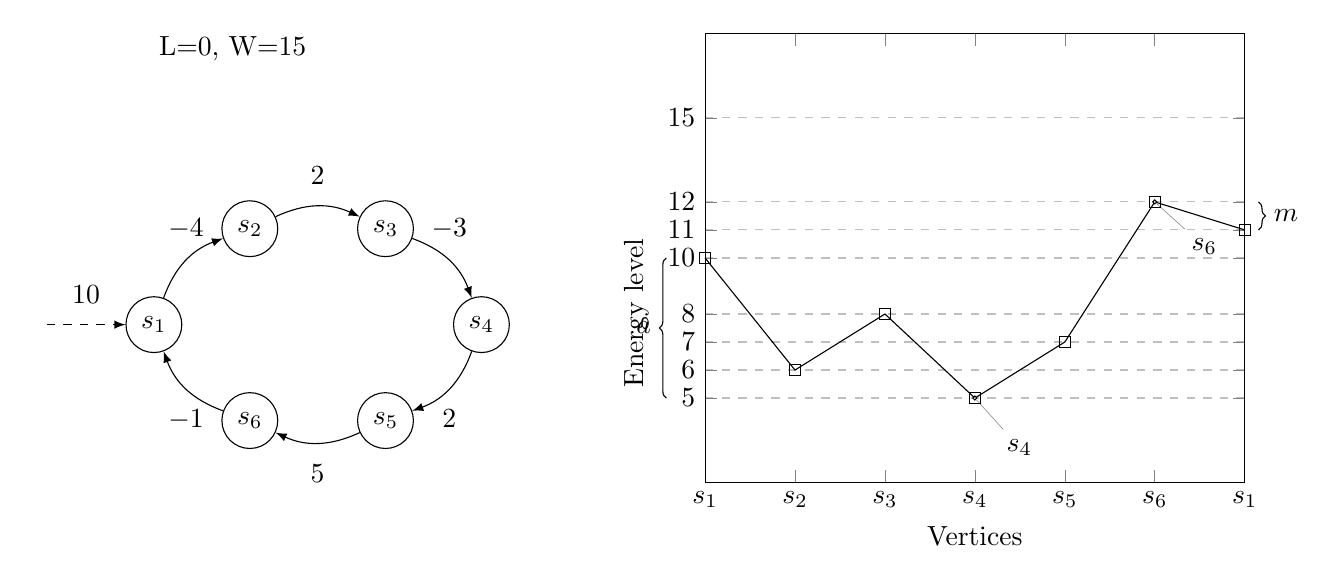
\begin{tikzpicture}[scale=1,auto ,node distance =1 cm,
state/.style ={ circle,draw}]
    \begin{scope}[yshift=-2cm]
    \node[state] (A) [] {$s_1$};
\node[state] (B) [above right=of A] {$s_2$};
\node[state] (C) [right=of B] {$s_3$};
\node[state] (D) [below right=of C] {$s_4$};
\node[state] (E) [ below left=of D] {$s_5$};
\node[state] (F) [left=of E] {$s_6$};
\node (01) [left =of A] {$$};
\path (1,3.5) node[text width=4cm,align=center] {L=0, W=15};

\path (01) edge [-latex,dashed] node[above =0.15 cm] {$10$} (A);
\path (A) edge [-latex,bend left =25] node[above =0.15 cm] {$-4$} (B);
\path (B) edge [-latex,bend left =25] node[above =0.15 cm] {$2$} (C);
\path (C) edge [-latex,bend left =25] node[above =0.15 cm] {$-3$} (D);
\path (D) edge [-latex,bend left =25] node[below =0.15 cm] {$2$} (E);
\path (E) edge [-latex,bend left =25] node[below =0.15 cm] {$5$} (F);
\path (F) edge [-latex,bend left =25] node[below =0.15 cm] {$-1$} (A);
    \end{scope}
%
    \begin{scope}[xshift=7cm, yshift=-4cm]
    \begin{axis}[
    title={},
    xlabel={Vertices},
    ylabel style= {xshift=-20pt},
    ylabel={ Energy level},
    clip=false,
    xmin=1, xmax=7,
    ymin=2, ymax=18,
    xtick={1,2,3,4,5,6,7},
    ytick={5,6,7,8,10,11,12,15},
    xticklabels={$s_1$,$s_2$,$s_3$,$s_4$,$s_5$,$s_6$,$s_1$},
     legend pos=north east,
    ymajorgrids=true,
    grid style=dashed,
]

\addplot[
    color=black,
    mark=square,
    ]
    coordinates {
    (1,10)(2,6)(3,8)(4,5)(5,7)(6,12)(7,11)
    }; 

\node[inner sep=0.5pt,circle,draw,-latex,fill=white,pin=-55: $s_4$] 
	  at (axis cs:4,5) {};
	  \node[inner sep=0.5pt,circle,draw,-latex,fill=white,pin=-45: $s_6$] 
	  at (axis cs:6,12) {};


\draw[decorate,decoration={brace}]
  ([xshift=-14pt]axis cs:1,5) --
    node[left=2pt] { $a$} 
  ([xshift=-14pt]axis cs:1,10);

\draw[decorate,decoration={brace,mirror}]
  ([xshift=5pt]axis cs:7,11) --
    node[right=2pt] {$m$} 
  ([xshift=5pt]axis cs:7,12);
\end{axis}
      \end{scope}
  \end{tikzpicture}

\caption{Energy level of a positive cycle}

  \end{figure}
  \vskip 0.1cm
  In the example, $a=5$ and $m=1$, i.e. if player $1$ can reach $s_1$ with at least 5 energy level, she can rotate the cycle as much as she wants, and can increase the output energy level up to 14.\\
  
  Now, we express this intuition formally by proving a series of lemmas:\\
\vskip 1cm
\begin{lemma}
\label{lemma-higherrun}
Let $\pi$ be a finite path in a one-player arena~$G$. 
If $(q,u) \xrightarrow{\pi}_{LW} (q',u')$, then for any~$v\geq u$,
$(q,v) \xrightarrow{\pi}_{LW} (q',v')$ for some~$v'\geq u'$.
\end{lemma}

Notice that, even if we add condition~$u'>u$ in the
hypotheses of Lemma~\ref{lemma-higherrun}, it~need not be the case that
$v'>v$. In~other terms, a~sequence of transitions may have a positive
effect on the final energy level from some configuration, and a negative effect from another one, due to the weak upper bound limit.
%But we can prove the following lemmas:
Below, we prove a series of results related to this issue, and that
will be useful for the rest of the proof.

\vskip 0.5cm
\begin{lemma}
\label{lemma-hitW}
  Let $\pi$ be a finite path in a one-player arena~$G$, and consider two LW-runs $(q,u)\xrightarrow{\pi}_{LW} (q',u')$ and $(q,v)\xrightarrow{\pi}_{LW}(q',v')$ with $u\leq
  v$. Then $u'-u\geq v'-v$, and if the inequality is strict, then
  the energy level along the run $(q,v)\xrightarrow{\pi}_{LW}(q',v')$ must have hit~$W$.
\end{lemma}

\vskip 0.5cm
\begin{lemma}
\label{lemma-W}
  Let $\pi$ be a finite path in a one-player arena~$G$, for which there
  is an LW-runs $(q,u)\xrightarrow{\pi}_{LW} (q',u')$. 
  %with $u\leq u'$. (suppressed this info otherwise the second statement makes no sense) 
  If $u'$ is the maximal energy level along that run, then
  $(q,W)\xrightarrow{\pi}_{LW} (q',W)$;
  if $u$ is the maximal energy level along the run above, then
  $(q,W)\xrightarrow{\pi}_{LW} (q',W+u'-u)$.
\end{lemma}

\vskip 0.5cm
\begin{lemma}\label{lemma-iteratepos}
  Let $\pi$ be a finite path in a one-player arena~$G$.
  If
  $(q,u)\xrightarrow{\pi}_{LW} (q',u')$ with $u'> u$
  and 
  $(q,w)\xrightarrow{\pi}_{LW} (q',w')$ with $w'> w$,
  then
  for any $u\leq v\leq w$, it~holds
  $(q,v)\xrightarrow{\pi}_{LW} (q',v')$ with $v'> v$.
\end{lemma}

From Lemma~\ref{lemma-higherrun}, it~follows that any run witnessing
LW-energy reachability can be assumed to contain no cycle with
non-positive effect. Formally:

\vskip 0.5cm
\begin{lemma}
\label{lemma-removeneg}
  Let $\pi$ be a finite path in a one-player arena~$G$.
  If $(q,u) \xrightarrow{\pi}_{LW} (q',u')$ and $\pi$ can be decomposed as
  $\pi_1\cdot\pi_2\cdot \pi_3$ in such a way that
  $(q,u) \xrightarrow{\pi_1}_{LW}
  (s,v)\xrightarrow{\pi_2}_{LW}(s,v') \xrightarrow{\pi_3}_{LW}(q',u')$ with $v'\leq
  v$, then $(q,u)\xrightarrow{\pi_1\cdot\pi_3}_{LW} (q',u'')$ with $u''\geq
  u'$.
\end{lemma}


The following lemma states that any LW-feasible cycle with
non-negative effect can be iterated, and that the energy level reached after a certain number of  iterations
eventually converges.
\vskip 0.5cm
\begin{lemma}\label{lemma-iteratecycles}
  Let $\pi$ be a cycle on~$q$ such that $(q,u) \xrightarrow{\pi}_{LW} (q,v)$
  for some $u\leq v$. Then $(q,u) \xrightarrow{\pi^{W-L}}_{LW} (q,v')$ for
  some~$v'$, and $(q,v')\xrightarrow{\pi}_{LW} (q,v')$.
\end{lemma}


Fix a path~$\pi$ in~$G$, and assume that some cycle~$\phi$ appears
(at~least) twice along~$\pi$: the~first time from some
configuration~$(q,u)$ to some configuration~$(q,u')$, and the second
time from~$(q,v)$ to~$(q,v')$. First, we~may assume that $\phi$ has
length at most~$|Q|$, since otherwise we can take an inner
subcycle.  We~may also assume that $v>u'$, as otherwise we~can apply
Lemma~\ref{lemma-removeneg} to get rid of the resulting non-positive cycle between~$(q,u')$ and~$(q,v)$. For the same reason we may assume
$u'>u$ and $v'>v$.  As~a consequence, by Lemma~\ref{lemma-iteratepos},
by repeatedly iterating~$\phi$ 
from~$(q,u)$, we~eventually reach some
configuration~$(q,w)$ with $w\geq v'$, from which we can follow the
suffix of~$\pi$ after the second occurrence of~$\phi$. It~follows that
all~occurrences of~$\phi$ along~$\pi$ can be grouped together, and
we~can restrict our attention to runs of the form $\alpha_1\cdot
\phi_1^{n_1}\cdot \alpha_2\cdot\phi_2^{n_2}\cdots
\phi_k^{n_k}\cdot\alpha_{k+1}$ where the cycles~$\phi_j$ are distinct
and have size at most~$|Q|$, and the finite runs~$\alpha_j$ are
acyclic.  Notice that by Lemma~\ref{lemma-iteratecycles}, we~may
assume $n_j=W-L$ for all~$j$.




While this allows us to only consider paths of a special form, this
does not provide \emph{short} witnesses, since there may be
exponentially many cycles of length less than or equal to $|Q|$,
and the witnessing run may need to iterate several cycles looping on
%the same state (see~Example~\ref{ex-cycles}). 
the same state (see~Example~\ref{ex-LW}).
In~order to circumvent this problem, we have to show that all cycles need not be considered, and that one 
can compute the "useful" cycles efficiently. 
For this, we first
introduce \emph{universal} cycles, which are cycles
that can be iterated from any initial energy level greater than the lower bound $L$.

\vskip 0.7cm
\begin{definition}
A \emph{universal cycle} on~$q$ is a cycle~$\phi$ with
$first(\phi)=last(\phi)=q$ such that $(q,L)\xrightarrow{\phi}_{LW}(q,v_{\phi,L})$ for some~$v_{\phi,L}$. A universal cycle is \emph{positive} if $v_{\phi,L}>L$
\end{definition}

\vskip 0.4cm
Note that, when a cycle $\phi$ is iterated $W-L$ times in a row, then some universal cycle $\sigma$ is also iterated $W-L-1$ times (by~considering the state with minimal energy level along~$\phi$). 
In figure~\ref{unicycle}, $abcde$ is not a universal cycle as it can not be iterated from initial energy level 0, but $bcdea$ is a universal one as it can be iterated infinitely from initial energy level 0. Also, note that $b$ is actually the lowest point of the cycle.

\begin{figure}[htb]
    \centering
  \begin{tikzpicture}[scale=1.1]
    \begin{scope}
    \draw (-2,0) node[rond5,jaune] (a) {} node {$a$};
    \draw (0,2) node[rond5,jaune] (b) {} node {$b$};
    \draw (2,0) node[rond5,jaune] (c) {} node {$c$};
    \draw (1,-2) node[rond5,jaune] (d) {} node {$d$};
    \draw (-1,-2) node[rond5,jaune] (e) {} node {$e$};
    
    \draw (a) edge[-latex',vert] node[left] {$-1$} (b);
    \draw (b) edge[-latex',vert] node[left] {$3$} (c);
    \draw (c) edge[-latex',vert] node[left] {$-1$} (d);
    \draw (d) edge[-latex',vert] node[below] {$3$} (e);
    \draw (e) edge[-latex',vert] node[left] {$-1$} (a);
    \draw (e) edge[-latex'] node[left] {$-3$} (b);
    \draw (b) edge[-latex'] node[left] {$2$} (d);
    \end{scope}
\end{tikzpicture}
\caption{Universal Cycles: abcde is not universal but bcdea is}

  \label{unicycle}
\end{figure}
    
    

Hence, every cycle can be replaced by a universal cycle. As~a consequence, iterating only universal cycles is enough: we~may now only look for runs of the form $\beta_1\cdot \sigma_1^{n_1}\cdot \beta_2\cdot\sigma_2^{n_2}\cdots
\sigma_k^{n_k}\cdot\beta_{k+1}$ where ~$\sigma_j$'s are \emph{universal} cycles
of length at most~$|Q|$. Now, assume that some state~$q$ admits
two universal cycles~$\sigma$ and~$\sigma'$, and that both cycles
appear along a given run~$\pi$. Write~$e$ (resp.~$e'$) for the energy
levels reached after iterating~$\sigma$ (reap.~$\sigma'$) $W-L$
times. We~define an order on universal cycles of~$q$ by letting
$\sigma \triangleright \sigma'$ when $e>e'$.  Then if~$\sigma \triangleright
\sigma'$, each occurrence of~$\sigma'$ along~$\pi$ can be replaced
with~$\sigma$, yielding a run~$\pi'$ that still satisfies the LW-energy condition (and~has the same first and last states). in figure \ref{unicycle}, both $bcdea$ and $bde$ are universal cycles on the vertex $b$. But, for $bcdea$, output energy is 2 while for $bde$ it is 1. Hence, $bcdea \triangleright bde$.\\
%
Generalizing this argument, each state that admits universal cycles has an optimal universal cycle
of length at most~$|Q|$, and it is enough to iterate only this
universal cycle to find a path witnessing reachability. This provides us with a \emph{small witness}, of the form $\gamma_1\cdot
\tau_1^{W-L}\cdot \gamma_2\cdot\tau_2^{W-L}\cdots
\tau_k^{W-L}\cdot\gamma_{k+1}$ where $\tau_j$ are optimal universal
cycles of length at most~$|Q|$ and $\gamma_j$ are acyclic
paths. Since it~suffices to consider at most one universal cycle per state, we~have $k\leq |Q|$.
%
From this, we~immediately derive an NP algorithm for solving
LW-energy reachability for one-player arenas: it~suffices to
non-deterministically select each portion of the path, and compute
that each portion is LW-feasible (notice that there is no need for
checking universality nor optimality of cycles; those properties were only used to prove that small witnesses exist). Checking
LW-feasibility requires computing the final energy level reached after iterating a cycle $W-L$ times; this can be performed by detecting the highest energy level along that cycle, and computing how much the energy level decreases from that point on until the end of the
cycle.

  \vskip 0.1cm
  We~now prove that optimal universal cycles of length at most~$|Q|$ can be computed for a given state~$q_0$. For~this we unwind the graph from~$q$ as a DAG of depth~$|Q|$, so that it includes all cycles of length at most~$|Q|$. We~name the states of this DAG $[q',d]$ (using square brackets to avoid confusion with configurations~$(q,l)$ where $l$ is the energy level) where $q'$ is the name of a state of the arena and $d$ is the depth of this state; hence there are transitions $([q',d],w,[q'',d+1])$ in the DAG as soon as there is a transition $(q',w,q'')$ in the arena.
  
    We~then explore this DAG from its initial state~$[q_0,0]$,
    looking for (paths corresponding~to) universal cycles. Our~aim is to keep track of all runs from~$[q_0,0]$ to~$[q',d]$ that are prefixes of universal cycles starting from~$q_0$. Actually, we~do not need to keep track of those runs explicitly, and it suffices for each such run to remember the following two values:
    \begin{itemize}
    \item the maximal energy level~$M$ that has been observed along the run so~far (starting from energy level~$L$, with weak upper bound~$W$);
    \item the difference~$m$ between the maximal energy level~$M$ and the final energy level in~$[q',d]$. Notice that~$m\geq 0$, and that the final energy level in~$[q',d]$ is~$M-m$. 
    \end{itemize}
    
    Figure~\ref{fig-ex_cycles} shows two example cycles. The first one ends with $M_1=5, m_1=4$, i.e. with an energy level of $1$. The second cycle has a maximal energy level $M_2=4$ and ends with $m_2=2$. Hence, iterating this cycle, one can end in state $q_0$ with energy level $\wub-m_2=3$.
    
    \begin{figure}[htbp]
        \centering
        \scalebox{1}{
          \begin{tikzpicture}
  \begin{scope}
    \draw (0,0) node[rond,rouge] (q0) {} node {$q_0$};
    \draw (2,0) node[rond,jaune] (q1) {} node {$q_1$};
    \draw (2,1.5) node[rond,jaune] (q2) {} node {$q_2$};
    \draw (0,1.5) node[rond,jaune] (q3) {} node {$q_3$};
    \draw (4,0) node[rond,jaune] (q4) {} node {$q_4$};
     \draw (2,3) node[rond,jaune] (q5) {} node {$q_5$};
    \draw (q0) edge[-latex'] node[below] {$+2$} (q1)
    (q1) edge[-latex'] node[above left] {$+5$} (q2)
    (q2) edge[-latex'] node[above] {$-3$} (q3)
    (q3) edge[-latex'] node[below left] {$-2$} (q0)
    (q1) edge[-latex'] node[above] {$-1$} (q4)
    (q4) edge[-latex'] node[below right] {$+2$} (q5)
    (q5) edge[-latex', bend right] node[below] {$+1$} (q3);  
    
    \end{scope}
    \begin{scope}
    \begin{scope}[scale=0.7,xshift=8cm,yshift=-1cm]
\draw[->] (-0.2,0) -- (6.5,0) node[right] {$\sharp steps$};
\draw[->] (0,-0.2) -- (0,6) node[above] {$M$};

\foreach  \x in {1,2,3,4,5}{
\draw[] (\x,-0.2) -- (\x,0.2){};
}

\foreach  \y in {1,2,3,4,5}{
\draw[] (-0.2,\y) -- (0.2,\y){};
}

\draw[dashed] (0,5) -- (5.5,5){};
\node (lh) at (-1,5) {$\wub$};

\tikzstyle{noeud}=[fill=white,draw,circle,inner sep=0pt,minimum width=5mm]

\node[] (l0) at (0,-0.8) {$0$};
\node [noeud](p0) at (0,0) {$q_0$};

\node[] (l1) at (1,-0.8) {$1$};
\node [noeud](p1) at (1,2) {$q_1$};
\draw[] (p0)--(p1){};

\node[] (l2) at (2,-0.8) {$2$};
\node [noeud](p2) at (2,5) {$q_2$};
\draw (p1)--(p2){};

\node[] (l3) at (3,-0.8) {$3$};
\node [noeud](p3) at (3,2) {$q_3$};
\draw (p2)--(p3){};

\node[] (l4) at (4,-0.8) {$4$};
\node [noeud](p4) at (4,1) {$q_0$};
\draw (p3)--(p4){};

\node [noeud](p5) at (2,1) {$q_4$};
\draw [color=red]  (p1)--(p5){};

\node [noeud](p6) at (3,3) {$q_5$};
\draw [color=red] (p5)--(p6){};

\node [noeud](p7) at (4,4) {$q_3$};
\draw [color=red] (p6)--(p7){};

\node[] (l5) at (5,-0.8) {$5$};
\node [noeud](p8) at (5,2) {$q_0$};
\draw [color=red] (p7)--(p8){};


\end{scope}

    \end{scope}  
      \end{tikzpicture}
  


        }
        \caption{Two cycles with upper bound $\wub=5$}
        \label{fig-ex_cycles}
    \end{figure}
    
    
    
    If~we know the values~$(M,m)$ of some path from~$[q_0,0])$ to~$[q',d]$, we~can decide if a given transition with weight~$w$ from~$[q',d]$ to~$[q'',d+1]$ can be taken 
    (the resulting path can still be a prefix of a universal cycle if $M-m+w \geq L$ ), and how the values of~$M$ and~$m$ have
    to be updated: if $w>m$, the~run will reach a new maximal energy level, and the new pair of values is $(min(W;M-m+w),0)$; if $m+L-M\leq w\leq m$, then the transition can be taken: the new energy level~$M-m+w$ will remain between~$L$ and~$M$, and we update the pair of values to~$(M,m-w)$; finally, if $w<m+L-M$, the energy level would go below~$L$, and the resulting run would not be a prefix of a universal cycle.
    
    
    Following these ideas, we inductively attach to states of the DAG sets of labels:
    initially, $[q_0,0]$ is labelled with~$(M=L,m=0)$; then if a
    state~$[q',d]$ is labelled with~$(M,m)$, and if there is a transition from~$[q',d]$ to~$[q'',d+1]$ with weight~$w$:
    \begin{itemize}
    \item if $w>m$, then we~label $[q'',d+1]$ with the pair $(\max(W;M-m+w),0)$;
    \item if $m+L-M\leq w\leq m$, we label $[q'',d+1]$ with $(M,m-w)$.
    \end{itemize}
    
    \begin{lemma}
    \label{lemma-DAGlabel}
    Let~$[q,d]$ be a state of the DAG, and $M$ and~$m$ be two integers
    such that $0\leq m\leq M$.  Upon termination of this algorithm,
    state~$[q,d]$ of the DAG is labelled with~$(M,m)$ if, and only if, there is an LW-run of length~$d$ from~$(q_0,L)$ to~$(q,M-m)$ along which the energy level always remains in the interval~$[L,M]$.
    \end{lemma}
    
    \begin{lemma}
    \label{lemma-univcycle}
    Let~$[q_0,d]$ be a state of the DAG, with~$d>0$. Let $m$ be a
    non-negative integer such that $L<W-m$.  Upon termination of this algorithm, state~$[q_0,d]$ is labelled with~$(M,m)$ such that $M-m>L$ if, and only if, there is a universal positive cycle~$\phi$ on~$q_0$ of length~$d$ such that $(q_0,L) \xrightarrow{\phi^{W-L}}_{LW} (q_0,W-m)$.
    \end{lemma}
    
    
    The algorithm above computes optimal universal cycles, but it still runs in exponential time (in the worst case) since it may generate exponentially many different labels in each state~$[q,d]$ (one per path from~$[q_0,0]$ to~$[q,d]$). We~now explain how to only generate polynomially-many pairs~$(M,m)$. This is based on the following partial order on labels: we~let $(M,m) \preceq (M',m')$ whenever $M-m\leq M'-m'$ and $m'\leq m$. Notice in particular that
    \begin{itemize}
    \item if~$M=M'$, then $(M,m)\preceq (M',m')$ if, and only~if, $m'\leq m$;
    \item if $m=m'$, then $(M,m)\preceq (M',m')$ if, and only~if, $M\leq M'$.
    \end{itemize}
    We~then have the following lemma:
    
    \vskip 0.5cm
    \begin{lemma}
    \label{lemma-order-cycle}
    Consider two paths~$\pi$ and~$\pi'$ such that
    $first(\pi)=first(\pi')$ and $last(\pi)=last(\pi')$, and with
    respective values~$(M,m)$ and~$(M',m')$ such that $(M,m)\preceq (M',m')$.
    If~$\pi$ is a prefix of a universal cycle~$\phi$, then $\pi'$~is a
    prefix of a universal cycle~$\phi'$ with $\phi'\triangleright \phi$.
    \end{lemma}
    
    
    In our algorithm above, it~suffices to keep track of the maximal labels for $\preceq$, since our aim is to compute optimal universal cycles. It~remains to prove that this way, we only store a polynomial number of labels:
    
    \vskip 0.5cm
    \begin{lemma}
    \label{lemma-DAG-construction-poly}
    If the DAG construction only stores maximal labels (for~$\preceq$), then it runs in polynomial time.
    \end{lemma}
    \vskip 0.3cm
    
    
    Using the algorithm above, we can compute, for each state~$q$ of the
    original arena, the~smallest value~$m_q$ for which there exists a
    universal cycle on~$q$ that, when iterated sufficiently many times,
    leads to configuration~$(q,W-m_q)$. Since universal cycles can be
    iterated from any energy level, if $q$ is reachable, then it is
    reachable with energy level~$W-m_q$. We~make this explicit by adding
    to our arena a special self-loop on~$q$, labelled with~$set(W-m_q)$,
    which sets the energy level to~$W-m_q$ (in~the same way as
    \emph{recharge transitions} of~\cite{EjsingDuun2013InfiniteRI}).
    
    In~the resulting arena, we know that we can restrict to paths of the
    form $\gamma_1\cdot \nu_1\cdot \gamma_2\cdot\nu_2\cdots
    \nu_k\cdot\gamma_{k+1}$, where $\nu_i$ are newly added transitions labelled with~$set(W-m)$, and $\gamma_i$ are acyclic paths. Such paths have length at most~$(|Q|+1)^2$. We~can then inductively compute the maximal energy level that can be reached (under our LW-energy constraint) in any state after paths of length less than or equal to~$(|Q|+1)^2$.  This can be performed by unwinding (as~a~DAG) the modified arena from the source state~$\qinit$ up to depth~$(|Q| +1)^2$, and labelling the states of this DAG by the maximal energy level with which that state can be reached from~$(\qinit,L)$; this is achieved in a way similar to our algorithm for computing the effect of universal cycles, but this time only keeping the maximal energy level that can be reached (under LW-energy constraint). As there are at most $|Q|$ states per level in this DAG of depth at most $(|Q|+1)^2$.\\
    This completes the proof for our theorem.
    \end{proof}
    \vskip 0.1cm
    Now, let's look at the following example:
    \begin{example}  
    Consider the one-player arena of Fig.~\ref{fig-ex}. We~assume $L=0$, and fix an even  weak upper bound~$W$. 
    %
    The~state~$s$ has $W/2$ disjoint cycles: for~each odd integer~$i$ in $[0;W-1]$, the~cycle~$c_i$ is made of three consecutive edges with weights $-i$, $+W$ and $-W+i+1$. Similarly, the~state~$s'$ has $W/2$ disjoint cycles: for even integers~$i$ in~$[0;W-1]$, the cycle~$c'_i$ has weights $-i$, $+W$ and~$-W+i+1$.  Finally, there are: two sequences of $k$ edges of weight~$0$ from~$s$ to~$s'$ and from~$s'$ to~$s$; an edge from the initial state to~$s$ with weight~$1$; an edge from~$s'$ to the target state with weight $-W$. The total number of states then is $2W+2k+2$.
    
    In order to go from the initial state, with energy level~$0$ to the final state, we have to first take the cycle $c_1$ (with weights~$-1$, $+W$, $-W+2$) on~$s$ (no~other cycles~$c_i$ can be taken). We~then reach configuration~$(s,2)$. Iterating~$c_1$ would have no effect, and the only next interesting cycle is~$c_2$, for which we~have to go to~$s'$. After running~$c_2$< we~end up in~$(s',3)$. Again, iterating~$c_2$ has no effect, and we go back to~$s$, take~$c_3$, and so~on. We~have to take each cycle~$c_i$ (at~least) once, and take the sequences of~$k$ edges between~$s$ and~$s'$ $W/2$ times each. In~the~end, we~have a run of length $3W+Wk+2$. 
    \vskip 0.5cm
    \begin{figure}[h]
      \centering
    \scalebox{1}{
      \begin{tikzpicture}
        \draw (0,0) node[rond,vert] (a) {} node {$s$};
        \draw (5,0) node[rond,vert] (b) {} node {$s'$};
        \draw (a) edge[bend left,-latex'] node[above] {$k$ edges} node[below] {weight=$0$} (b);
        \draw (b) edge[bend left,-latex'] node[above] {$k$ edges} node[below] {weight=$0$} (a);
        \draw (a) edge[out=160,in=200,looseness=9,-latex'] node[left] {$\genfrac{}{}{0pt}{0}{-i;+W;-W+i+1}{(\text{$i$ odd})}$} (a);
        \draw (b) edge[out=-20,in=20,looseness=9,-latex'] node[right] {$\genfrac{}{}{0pt}{0}{-i;+W;-W+i+1}{(\text{$i$ even})}$} (b);
      \end{tikzpicture}
      }
      \vspace{-2\medskipamount}
      \caption{An example showing that more than one cycle per state can be needed.}\label{fig-ex}
    \end{figure}
    \vskip 0.4cm
    Let us look at the universal cycles that we have in this arena:
    besides the cycles made of the $2k$ edges with weight~zero between~$s$ and~$s'$, the only possible universal cycles can only depart from the first state of each cycle~$c_i$ (as there are the only states having a positive outgoing edge). As~we proved, such cycles can be iterated arbitrarily many times, and set the energy level to some value in~$[L;w]$. Since the only edge available at the end of a universal cycle has weight~$+W$, the exact value of the universal cycles is unimportant: the energy level will be~$W$ anyway when reaching the second state of each cycle~$c_i$. As~a consequence, using set-edges
    in this example does not shorten the witnessing run, which then cannot be shorter than~$3W+Wk+2$ (which is more than $2|Q|$ but less than~$|Q|^2$). This demonstrates that we cannot avoid looking for quadratic-size runs in the modified arena at the end of our algorithm.
    \end{example}

    Now, we will move to the case for the two player version.

 
\section{Two Player QR Games with Weak Dual Bounds}

    Now, $Q_2 \not = \phi$ anymore. We~begin with proving a result
    similar to Lemma~\ref{lemma-higherrun}:
    \begin{lemma}
    \label{lemma-higherstrat}
      Let $G$ be a two-player arena, equipped with an \LWenergy-reachability
      objective. Let~$q$ be a state of~$G$, and~$u\leq u'$ in $[L;W]$. If
      \Pl1 wins the game from~$(q,u)$, then she also wins from~$(q,u')$.
    \end{lemma}
    
    By Martin's theorem~\cite{Mar75}, our games are determined. It~follows that if \Pl2 wins from
    some configuration~$(q,v)$, she also wins from~$(q,v')$ for
    all~$L\leq v'\leq v$ (assuming the contrary, i.e. $(q,v')$ winning for \Pl1, would lead to the contradictory statement that $(q,v)$ is both winning for \Pl1 and \Pl2). We~now prove that \Pl1 may need exponential memory, while \Pl2 can play
    memoryless strategies:
    \vskip 0.5cm
    \begin{lemma}
    \label{mem-lemma}
    For two player QR games with weak dual bounds, exponential memory may be necessary for player $1$. For player $2$, memoryless strategies are sufficient.
    \end{lemma}
    \begin{proof}
    As reachability is one of the objective, trivially finite memories are sufficient for both the players. Now, we will show, a class of game graphs, where exponential memory may be necessary for player $1$.\\
    \begin{figure}[htb]
    \centering
    \begin {tikzpicture}[-latex ,auto ,node distance =1 cm,
state/.style ={ circle, draw, minimum width =1 cm}]

\node[state] (A) [] {$q_0$};
\node[state] (B) [right=of A] {$v$};
\node[state] (C) [right=of B] {$T$};

\path (A) edge [] node[above =0.15 cm] {$U$} (B);
\path (B) edge [loop above] node[above =0.15 cm] {$-1$} (B);
\path (B) edge [] node[above =0.15 cm] {$U$} (C);
\end{tikzpicture}
\caption{Exponential memory is necessary for player $1$ }
    \label{expmem-p1}
    \end{figure}
    
    In the game graph of Figure \ref{expmem-p1}, all the vertices are player $1$  vertices, strong lower bound is $0$ while weak upper bound is $W$. It is easy to see, player $1$ needs at least $W$- memory to win this game. Considering binary encoding. the value of $W$ is exponential in the size of the input.\\
    \vskip 0.3cm
    Now, We~now prove that \Pl2 has memoryless optimal strategies. According
      to Lemma~\ref{lemma-higherstrat}, for each state~$q$, there is an
      integer $v_q\in[L;W+1]$ such that \Pl1 wins the game from any
      configuration~$(q,v)$ satisfying $v_q\leq v\leq W$, while \Pl2 wins
      the game from any configuration~$(q,v)$ with $L\leq v<v_q$.
    
      Assume that \Pl2 wins the game from some state~$(q,v)$, with $L\leq
      v\leq v_q$. Denote with\\~$(q,p_i,q_i)_{1\leq i\leq m}$ for the set of
      outgoing transitions from~$q$. By~definition of~$v_{q_i}$, \Pl1 wins
      the game from any configuration of the form~$(q_i,v)$ with $v\geq
      v_{q_i}$. Since \Pl2 wins from~$(q,v)$, there must exist an
      index~$1\leq i\leq m$ such that $v+p_i\leq v_{q_i}$. This defines a
      winning move for \Pl2 from~$(q,v)$. The~same argument applies in all
      states, and yields a memoryless winning strategy for \Pl2.
    \end{proof}
    \vskip 0.2cm
    
    Now, based on the previous lemma we can conclude the following theorem:\\
    \begin{theorem}
    \label{two-player-weak-thm}
    Given a game graph $G$ , a strong upper bound $U$ and a lower weak bound $0$, deciding if $P_1$ can win the 2 player QR games with weak dual bound game in $G$ is in $coNP$.
    \end{theorem}
    \begin{proof}
    A priori, lemma \ref{mem-lemma} says if $P_2$ has a winning strategy, he has a memoryless one. Now, we can guess a strategy for Player $2$ (i.e. select one transition per state in $Q_2$) and verify that this strategy is winning for Player $2$ by solving the one player game, which has been proved to be in polynomial time in theorem \ref{one-player-weak-thm}.
    \end{proof}
\vskip 0.5cm
% \section{A step towards NP}
% Now, we prove the existence of a small certificate for the strategy of player $1$. We have already shown that in the original game, player $1$ might need exponential memory. Now, we construct the exponential size graph $G^{\prime}$ with vertices $\langle q_i, E_i \rangle$ explicitly keeping track of the energy level. There is a edge between $\langle q_i, E_i \rangle$ to $\langle q_j, E_j \rangle$ iff there is an edge from $q_i$ to $q_j$ with weight $E_j -E_i$ in the graph $G$, where $E_i, E_j \leq U$. We also add a dead state $q_{dead}$, where any time the energy level goes beyond the upper bound $U$, we move to a dead state. Now, in this exponential graph $G^{\prime}$, the objective of player $1$ is to reach $\langle T,E \rangle$ for some $E \leq U$ from $\langle q_0,0 \rangle$.\\
% Clearly, player $1$ has a memoryless strategy to win in $G^{\prime}$ iff he has a strategy to win in $G$. Primarily the idea is that, if player $1$ reaches a same state with same energy level in different paths, all the time he can play the same edge which is the "best" for him and that implies, if player $1$ can win in $G^{\prime}$, he can win memorylessly. Now, we will prove the following lemma:
% \begin{lemma}
% \label{NP-cert}
% For a vertex $q$ in $G$, if there exists $E$ and $E^{\prime} \in \mathbb{N}$ such that, in $G^{\prime}$ player $1$ has a memoryless winning strategy $\lambda$ from $\langle q, E \rangle$ and $\lambda^{\prime}$ from $\langle q, E^{\prime} \rangle$ where, $\lambda(\langle q, E \rangle) = \lambda^{\prime}(\langle q, E^{\prime} \rangle)$, then for every $\langle q,E^{\prime \prime} \rangle$ where $E \leq E^{\prime \prime} \leq E^{\prime}$, there exists a memoryless winning strategy $\lambda^{\prime \prime}$ for player $1$ such that,  $\langle q, E^{\prime} \rangle$ where, $\lambda(\langle q, E \rangle) = \lambda^{\prime \prime}(\langle q,E^{\prime \prime})=\lambda^{\prime}(\langle q, E^{\prime} \rangle)$.
% \end{lemma}
% \vskip 0.1cm
% \begin{proof}
% The lemma says simply that, if player $1$ can play same action $a$ from a vertex $q$ with energy level $E$ and $E^{\prime}$, then he can play the same action from $q$ with any energy level between $E$ and $E^{\prime}$. First thing to notice that, it may look like if player $1$ plays a memoryless winning strategy with action $b$ from some vertex $v$ with energy level $E$, then he can play $b$ from $v$ with any energy level $\leq E$ and win. But, this is not true.To see this consider the figure \ref{not_true}. Lets say, $U=4$. So, player $1$ can play self loop action from $\langle v,4 \rangle$ and then win. But, from $\langle v,0 \rangle$ he cannot play the self loop action and win with a memoryless strategy in the exponential graph.\\
% \begin{figure}[htb]
% \hskip 6cm
% \label{not_true}
% \begin {tikzpicture}[-latex ,auto ,node distance =1 cm,
state/.style ={ circle, draw, minimum width =1 cm}]

\node[state] (A) [] {$q_0$};
\node[state] (B) [right=of A] {$v$};
\node[state] (C) [right=of B] {$T$};

\path (A) edge [] node[above =0.15 cm] {$4$} (B);
\path (B) edge [loop above] node[above =0.15 cm] {$-1$} (B);
\path (B) edge [] node[above =0.15 cm] {$1$} (C);
\end{tikzpicture}
\caption{Player $1$ cannot play same memoryless strategy from $\langle v,4 \rangle$ and $\langle v,0 \rangle$}
% \end{figure}
% But from $\langle v,1 \rangle$ he can play the same action and win with a memoryless strategy. So, the lemma says, from $\langle v,3 \rangle$ and $\langle v,2 \rangle$ also, he can play the same self loop action and win with a memoryless strategy in the exponential graph.\\
% Now, we will go to the proof of the lemma. 
% \fcolorbox{blue}{red}{Trying to work out the proof.}
% \end{proof}
% \vskip 0.5cm
% Now, the previous lemma takes us to a step towards proving that the $2$ player QR game with weak dual bound is in NP. This is because, though the energy levels are exponential when expressed in binary, the number of actions player $1$ can take from each vertex is linear in size. Now, lemma \ref{NP-cert} suggests that, for a fixed vertex we can group energy levels into intervals from where we can take the same action, hence the number of groups in also at most linear in size.\\
% This works as our short certificate. Given a game graph $G$ with weak dual bounds objective, we can guess a grouping of energy levels to produce a game graph $G^{\prime \prime}$ with vertices as $\langle s, I\rangle$, where $s$ is a vertex in $G$ and $I$ is an interval of energy levels. Note that, $G^{\prime \prime}$ has at most $O(n^2)$ many vertices. After guessing the short certificate, the verification process will be to check reachability of $\langle T, I\rangle$ for any interval $I$ and target state $T$ from $\langle q_0, I^{\prime} \rangle$, with $I^{\prime}$ containing 0. But, we do not know, how to execute this verification process in polynomial time. 

\section{Conclusion}
In this chapter, we have showed that QR games with weak dual bounds are in $P$ for the single player case and is in $coNP$ for the two player case. We also believe that the two player version of the game is in $NP$. We have shown the short certificate for the problem, but unfortunately could not prove the verification part.\\
This ends all the QR game versions with bounds on weight functions. In the next chapter, we will introduce a new QR game, with a notion of bound on number of violations.
 
\chapter{Apna Game}
In the previous chapters, we have explored all kind of weighted games, where the weight functions were bounded. In this chapter, we will explore a new kind of a game. Here also, we have strong bounds on weights, but player $1$ can violate one of the bounds, w.l.o.g, say the upper bound. The number of vertices, he traverses along his path with weights higher than the upper bound are called \textbf{violations}. In this game, we have a bound on the number of violations. We call this bounded violations reachability game as \textit{Apna Game}. We formally define it in the following section.\\

\section{Description of the Game}
Consider a game graph $G=\langle Q_1, Q_2, E, w, q_0, T \rangle$, a lower bound $l$, an upper bound $U$ and a 

\chapter{Conclusion}
In this thesis, we have considered several variants of energy games. The first variant defines games with upper and lower bound constraints, combined with reachability or infinite runs objectives. 
The second variant proposed defines games with a strong lower bound and a relaxed upper bound that can be weak or temporarily exceeded, combined with reachability or infinite run objectives, and constraints on violations of upper bound. 
\vskip 0.3cm
In the one player case, complexities ranges from PTIME to PSPACE-Complete. and in the two-player case from NP $\cap$ coNP to EXPTIME-Complete. 
In general, the complexity is the same for a reachability and for an infinite run objective. Interestingly, for \LWenergy games, the complexity of the single player case is PTIME, but reachability objectives require exponential memory (in the size of the weak upper bound) while strategies are memoryless for infinite run objectives.
\vskip 0.3cm
Table~\ref{table-results} summarizes known
results, and the results obtained in this paper (where \LVenergyall
gathers all three energy constraints with violations). We furthermore show that the minimization problem for \LVenergyall (reachability) games require algorithms that run in PSPACE in the one-player case, and in EXPTIME in the two-players case.


\begin{table}[ht]
  \centering
  \def\arraystretch{2}
  \def\comp{c.}
  \scalebox{0.7}{
  \begin{tabular}{|c||c|c||c|c|}
    \hline
    &\multicolumn{2}{c|}{Reachability}&\multicolumn{2}{c|}{Infinite runs}\\
    \hline
    & 1 player & 2 players & 1 player & 2 players
    \\\hline\hline
    \Lenergy & PTIME~(thm.~\ref{thm_reachability_games})&NP$\cap$ coNP~(thm.~\ref{thm_reachability_games}) 
    & PTIME~\cite{BouyerFLMS08} & in NP $\cap$ coNP~\cite{BouyerFLMS08}\\\hline
    %LUEnergy Games
    \LUenergy&PSPACE-\comp~(thm.~\ref{pspace-complete})& EXPTIME-\comp ~(thm.~\ref{exp-complete})
    & PSPACE-\comp~\cite{BouyerFLMS08} &EXPTIME-\comp~\cite{BouyerFLMS08}\\\hline
    %
    \LWenergy&PTIME~(thm.~\ref{one-player-weak-thm})&coNP~(thm.~\ref{two-player-weak-thm}) 
    &PTIME~\cite{BouyerFLMS08} &NP $\cap$ coNP~\cite{BouyerFLMS08}\\\hline
    %
    APNA$^{*}$-games &PSPACE-\comp~(thm.~\ref{thm_apna_LUHV_2P}) &EXPTIME-\comp~(thm.~\ref{thm_apna_LUHV_2P})&PSPACE-\comp~(thm.~\ref{thm_apna_LUHV_2P}) &EXPTIME-\comp~(thm.~\ref{thm_apna_LUHV_2P}) \\\hline
    
    
    Bound existence&PSPACE-\comp~(thm.~\ref{thm_Apnar_exists_min_exptimec})&EXPTIME-\comp~(thm.~\ref{thm_Apnar_exists_min_exptimec}) &PSPACE-\comp~(thm.~\ref{thm_Apnar_exists_min_exptimec})&EXPTIME-\comp~(thm.~\ref{thm_Apnar_exists_min_exptimec}) \\\hline
  \end{tabular}
  }
  \caption{Summary of the results}
  \label{table-results}
\end{table}
\vskip 1cm
A possible extension of this work is to consider energy games with mean payoff function and discounted total payoff for the energy level and for the violation constraints, and the associated minimization and existence problems. 




\bibliographystyle{alpha}
\bibliography{Thesis}

\appendix
\chapter{Appendix Title}
\section{Proofs of Section~\ref{sec-weak}}

\noindent{\bf Lemma \ref{lemma-higherrun}: }
  Let $\pi$ be a finite path in a one-player arena~$G$.
  If $(q,u) \xrightarrow{\pi}_{LW} (q',u')$,
  then for any~$v\geq u$,
  $(q,v) \xrightarrow{\pi}_{LW} (q',v')$ for some~$v'\geq u'$.

\begin{proof}
Write $\pi=(e_i)_{0\leq i<n}$, with $e_i=(q_i,p_i,q'_i)$ for each~$i$.
The sequence defined as
\begin{xalignat*}2
  u_0&= u & u_{i+1} &= \min{W,u_i+p_i}
\end{xalignat*}
is the sequence of energy levels along the run $(q,u) \xrightarrow{\pi}_{LW}
(q',u')$.  For~$v\geq u$, letting
\begin{xalignat*}2
  v_0&= v & v_{i+1} &= \min{W,v_i+p_i},
\end{xalignat*}
we~easily prove by induction that for all~$i$, $u_i\leq v_i\leq W$,
which entails that $(q,v) \xrightarrow{\pi}_{LW} (q',v')$ with $v'=v_n\geq
u_n=u'$.
\end{proof}


\noindent{\bf Proof of Lemma~\ref{lemma-hitW}}
  Let $\pi$ be a finite path in a one-player arena~$G$, and consider two LW-runs 
  $(q,u)\xrightarrow{\pi}_{LW} (q',u')$ and $(q,v)\xrightarrow{\pi}_{LW}(q',v')$ with $u\leq
  v$. Then $u'-u\geq v'-v$, and if the inequality is strict, then
  the energy level along the run $(q,v)\xrightarrow{\pi}_{LW}(q',v')$ must have hit~$W$.


\begin{proof}
  The first statement is proven by induction: we~again write
  $\pi=(e_i)_{0\leq i<n}$, with $e_i=(q_i,p_i,q'_i)$ for each~$i$, and
  \begin{xalignat*}2
    u_0&= u & u_{i+1} &= \min(W,u_i+p_i)\\
    v_0&= v & v_{i+1} &= \min(W,v_i+p_i).
  \end{xalignat*}
  Then $u_{i+1}-u_i=\min(W-u_i,p_i)$ and
  $v_{i+1}-v_i=\min(W-v_i,p_i)$.  Since $u_i\leq v_i$ for all~$i$,
  we~also have $W-u_i\geq W-v_i$, and $u_{i+1}-u_i \geq
  v_{i+1}-v_i$. By~summing up these inequalities, we~get $u_{i+1}-u_0
  \geq v_{i+1}-v_0$. Now, as long as $W-v_i\geq p_i$ (then also
  $W-u_i\geq p_i$), the inequalities above are equalities. It~follows
  that if the inequality is strict, then the run
  $(q,v)\xrightarrow{\pi}_{LW}(q',v')$ must have hit~$W$.
\end{proof}


\noindent{\bf Proof of Lemma~\ref{lemma-W}}
Let $\pi$ be a finite path in a one-player arena~$G$, for which there
  is an LW-runs $(q,u)\xrightarrow{\pi}_{LW} (q',u')$. 
  %with $u\leq u'$. (suppressed this info otherwise the second statement makes no sense) 
  If $u'$ is the maximal energy level along that run, then
  $(q,W)\xrightarrow{\pi}_{LW} (q',W)$;
  if $u$ is the maximal energy level along the run above, then
  $(q,W)\xrightarrow{\pi}_{LW} (q',W+u'-u)$.


\begin{proof}
  Write $\pi=(e_i)_{0\leq i<n}$, with $e_i=(q_i,p_i,q'_i)$ for
  each~$i$. If~$u'$ is the maximal energy level, then for all~$i$,
  we~have $\sum_{j=i}^{n-1} p_j\geq 0$.  Now, define
  \begin{xalignat*}2
    v_0&= W & v_{i+1} &= \min(W,v_i+p_i).
  \end{xalignat*}
  If~$v_n<W$, then by induction we also have $v_i<W$ for all~$i$,
  contradicting the fact that~$v_0=W$. This proves our first result.

  Similarly, if~$u$ is the maximal energy level, then for all~$i$,
  we~have $\sum_{j=0}^{i} p_j\leq 0$. Then for all~$i$,
  $v_{i+1}=v_i+p_i\leq W$, so that $v_{n}-v_0=u'-u$. Our second result
  follows.
\end{proof}


\noindent{\bf Proof of Lemma~\ref{lemma-iteratepos}}
Let $\pi$ be a finite path in a one-player arena~$G$.
  If
  $(q,u)\xrightarrow{\pi}_{LW} (q',u')$ with $u'> u$
  and 
  $(q,w)\xrightarrow{\pi}_{LW} (q',w')$ with $w'> w$,
  then
  for any $u\leq v\leq w$, it~holds
  $(q,v)\xrightarrow{\pi}_{LW} (q',v')$ with $v'> v$.

\begin{proof}  
Using Lemma~\ref{lemma-higherrun}, we~immediately have
$(q,v)\xrightarrow{\pi}_{LW} (q',v')$. As~in the previous proof, we~define
sequences
\begin{xalignat*}2
  u_0&= u & u_{i+1} &= \min(W,u_i+p_i)\\
  v_0&= v & v_{i+1} &= \min(W,v_i+p_i)\\
  w_0&= w & w_{i+1} &= \min(W,w_i+p_i).
\end{xalignat*}
We~still have $u_i\leq v_i\leq w_i$ for all~$i$. Moreover, 
%if $v_j<M$
if $v_j<\wub$
for all~$j\leq i$, then $v_i-u_i=v-u$. As~a consequence, if $v'\leq
v$, then it must be the case that 
%$v_j=M$ 
$v_j=\wub$ 
for some~$j$; but then $w_j=v_j$, 
%since $v_j\leq w_j\leq M$. 
since $v_j\leq w_j\leq \wub$. 
It~follows that $w_k=v_k$ for
all~$k\geq j$, so at the end of $\pi$ we have $w'=v'$. Assuming $v'\leq v$ raises a contradiction since we have $v'=w'>w\geq v$.
%This is a contradiction, since we assumed $v'\leq v$ and have $w'>w$ by hypothesis. 
Hence $v'>v$.
\end{proof}

\noindent{\bf Proof of Lemma~\ref{lemma-removeneg}}
Let $\pi$ be a finite path in a one-player arena~$G$.
  If $(q,u) \xrightarrow{\pi}_{LW} (q',u')$ and $\pi$ can be decomposed as
  $\pi_1\cdot\pi_2\cdot \pi_3$ in such a way that
  $(q,u) \xrightarrow{\pi_1}_{LW}
%  (s,v)\LWarrow{\pi_2}(s',v') \LWarrow{\pi_3}(q',u')$ with $v'\leq
  (s,v)\xrightarrow{\pi_2}_{LW}(s,v') \xrightarrow{\pi_3}_{LW}(q',u')$ with $v'\leq
  v$, then $(q,u)\xrightarrow{\pi_1\cdot\pi_3}_{LW} (q',u'')$ with $u''\geq
  u'$.

\begin{proof}
%Since $(s',v') \LWarrow{\pi_3}(q',u')$ and $v'\leq v$, by
Since $(s,v') \xrightarrow{\pi_3}_{LW}(q',u')$ and $v'\leq v$, by
Lemma~\ref{lemma-higherrun} 
%we also have $(s',v)
we also have $(s,v)
\xrightarrow{\pi_3}_{LW}(q',u'')$ for some~$u''\geq u'$. The~result follows.
\end{proof}


\noindent{\bf Proof of Lemma~\ref{lemma-iteratecycles}}
Let $\pi$ be a cycle on~$q$ such that $(q,u) \xrightarrow{\pi}_{LW} (q,v)$
  for some $u\leq v$. Then $(q,u) \xrightarrow{\pi^{W-L}}_{LW} (q,v')$ for
  some~$v'$, and $(q,v')\xrightarrow{\pi}_{LW} (q,v')$.


\begin{proof}
  The case where $u=v$ is trivial. We~assume $u<v$.  Applying
  Lemma~\ref{lemma-higherrun} inductively, we get that the cycle can
  be iterated arbitrarily many times; this~also proves that the
  sequence of energy levels reached at the end of each iteration is
  non-decreasing.

  Now, assume that $(q,v')\xrightarrow{\pi}_{LW} (q,v'')$ for
  some~$v''\not=v'$.  Then $v''>v'$. Lemma~\ref{lemma-iteratepos} then
  entails that the sequence of energy levels reached at the end of
  each iteration is increasing. Since the loop has been iterated $W-L$
  times, the~energy level in~$v''$ would exceed~$W$, which is
  impossible. This proves our result.
\end{proof}


\noindent{\bf Proof of Lemma~\ref{lemma-DAGlabel}}
  Let~$[q,d]$ be a state of the DAG, and $M$ and~$m$ be two integers
  such that $0\leq m\leq M$.  Upon termination of this algorithm, 
  state~$[q,d]$ of the DAG is labelled with~$(M,m)$ if, and only if,
  there is an LW-run of length~$d$ from~$(q_0,L)$ to~$(q,M-m)$ along
  which the energy level always remains in the interval~$[L,M]$.

\begin{proof}
  The proof is by induction on~$d$. The result is trivial for~$d=0$.
  Now, assume it holds for some depth~$d-1$, and pick a
  state~$[q,d]$. For the first direction, if~$[q,d]$ is labelled
  with~$(M,m)$, then this label was added using some
  transition~$([q',d-1],w,[q,d])$ and some label~$(M',m')$
  of~$[q',d-1]$. By~induction, there is an LW-run~$\rho$ of
  length~$d-1$ from~$(q_0,L)$ to~$(q',M'-m')$ in~$G$ along which the
  energy level remains in the interval~$[L,M']$. We~consider two cases,
  corresponding to the two ways of updating the pair of values:
  \begin{itemize}
  \item if $w>m'$, then we~have $M=min(\wub,M'-m'+w)$ and $m=0$. %$M=\max(W,M'-m'+w)$ and $m=0$. 
  Now, the transition $([q',d-1],w,[q,d])$ in the DAG originates from a
    transition~$(q',w,q)$ in~$G$; taking this transition after~$\rho$
    provides us with the run of length~$d$ from~$(q_0,L)$ to~$(q,M-m)$
    along which the energy level remains in~$[L,M]$, as required;
  \item if $m'+L-M'\leq w\leq m'$, then $M=M'$ and $m=m'-w$. Again,
    taking transition~$(q',w,q)$ after~$\rho$ provides us with the
    LW-run we are looking for.
  \end{itemize}

  Conversely, if there is an LW-run~$\rho$ of length~$d$
  from~$(q_0,L)$ to~$(q,M-m)$ along which the energy level always
  remains in the interval~$[L,M]$, then we~write $\rho=\rho'\cdot
  ((q',l'),w,(q,M-m))$, distinguishing its last transition. By~induction, $[q',d-1]$ must have been labelled with a pair~$(M',m')$ such that $l'=M'-m'$ and the energy level
  along $\rho'$ remained within $[L,M']$. Now, from the existence of a transition $((q',l'),w,(q,M-m))$, we~know that there is a
  transition~$([q',d-1],w,[q,d])$ in the~DAG, which will generate the required label of~$[q,d]$.
\end{proof}

\noindent{\bf Proof of Lemma~\ref{lemma-univcycle}}
  Let~$[q_0,d]$ be a state of the DAG, with~$d>0$. Let $m$ be a
  non-negative integer such that $L<W-m$.  Upon termination of this algorithm, state~$[q_0,d]$ is labelled with~$(M,m)$ such that $M-m>L$ if, and only if, there is a universal  positive cycle~$\phi$ on~$q_0$ of length~$d$ such that $(q_0,L) \xrightarrow{\phi^{W-L}}_{LW} (q_0,W-m)$.

\begin{proof}
First assume that~$[q_0,d]$ is labelled with~$(M,m)$ for some~$M$ such
that $M-m>L$. From Lemma~\ref{lemma-DAGlabel}, there is a cycle~$\phi$
on~$q_0$ of length~$d$ generating a run $(q_0,L)\xrightarrow{\phi}_{LW}(q_0,M-m)$
along which the energy level is within~$[L,M]$.  Then~$M-m\geq L$, so
that Lemma~\ref{lemma-iteratecycles} applies: we~then get $(q_0,L)
\xrightarrow{\phi^{W-L}}_{LW} (q_0,E)$ with $(q_0,E)\xrightarrow{\phi}_{LW}(q_0,E)$.
Write $(p_i)_{0\leq i<|\phi|}$ for the sequence of weights along~$\phi$.
Also write $\rho$ for the run $(q_0,L)\xrightarrow{\phi}_{LW}(q_0,M-m)$, and
$\sigma$ for the run $(q_0,E)\xrightarrow{\phi}_{LW}(q_0,E)$.

%Assume $L=M-m$: iterating~$\phi$ would not modify the energy level
%reached at the end of those cycles, so that we would have
%$L=W-m$. Since this is not the case, it~must be 
As $L<M-m$, then by Lemma~\ref{lemma-hitW}, it~must be the case that energy level~$W$ is
reached along~$\sigma$.  Write~$i_0$ and $j_0$ for the first and last
positions along~$\rho$ for which the energy level along~$\rho$ is~$M$.
That is, the subpath from index $0$ to index $i_0$ has growing energy level, and the subpath from $j_0$ to $|\rho|$ has a decreasing energy level. 
Assume $\tilde\sigma_{i_0}\not=W$: by~Lemma~\ref{lemma-higherrun},
we~must have $M=\tilde\rho_{i_0}\leq \tilde\sigma_{i_0}<W$.  Then for
all~$k\geq i_0$, $\sum_{l=i_0}^k p_l\leq 0$, and $\sum_{l=i_0}^{j_0}
p_l= 0$. Since $\tilde\sigma_{i_0}<W$, then also $\tilde\sigma_{k}<W$
for all~$k\geq i_0$. According to Lemma~\ref{lemma-hitW}, energy level $\wub$ is reached in $\sigma$, so 
%HERE 
there exists some~$k_0<i_0$ such that $\tilde\sigma_{k_0}=W$;
%$\tilde\rho_{k_0}<M$, 
However, as $i_0$ is the index of the first maximal value in $\rho$, we have $\tilde\rho_{k_0}<M$, and the energy level increases in run $\rho$ between $k_0$ and $i_0$. So according to Lemma~\ref{lemma-W}, we should have $\tilde\sigma_{i_0}<W$, which raises a contradiction.
Hence we proved $\tilde\sigma_{i_0}=W$; applying
the second result of Lemma~\ref{lemma-W}, we~get $E=W-m$.

\medskip
Conversely, if there is a universal positive cycle~$\phi$ satisfying the
conditions of the lemma, let $F$ be such that $(q_0,L)\xrightarrow{\phi}_{LW}
(q_0,F)$, and~$M$ be the the maximal energy level encountered along
the run $(q_0,L)\xrightarrow{\phi}_{LW} (q_0,F)$. By
Lemma~\ref{lemma-DAGlabel}, state~$[q_0,d]$ is labelled with~$(M,m')$
for some~$m'\geq 0$ such that $F=M-m'$.
By~Lemma~\ref{lemma-iteratecycles}, we~must have $(q_0,L)
\xrightarrow{\phi^{W-L}}_{LW} (q_0,W-m')$.
%, so that $m'=m$.
\end{proof}


\noindent{\bf Proof of Lemma~\ref{lemma-order-cycle}}
Consider two paths~$\pi$ and~$\pi'$ such that
$first(\pi)=first(\pi')$ and $last(\pi)=last(\pi')$, and with
respective values~$(M,m)$ and~$(M',m')$ such that $(M,m)\preceq (M',m')$.
If~$\pi$ is a prefix of a universal cycle~$\phi$, then $\pi'$~is a
prefix of a universal cycle~$\phi'$ with $\phi'\triangleright\phi$.

\begin{proof}
  Let $q=first(\pi)$ and $q'=last(\pi)$.  We~write~$\psi$ for the
  path such that $\phi=\pi\cdot\psi$; $\psi$~is a path from~$q'$
  to~$q$. Then $(q,L)\xrightarrow{\pi}_{LW} (q'',M-m)
  \xrightarrow{\psi}_{LW}(q',F)$. Also, $(q,L)\xrightarrow{\pi}_{LW} (q'',M'-m')$.  Since
  $M-m\leq M'-m'$, we have $(q'',M'-m')\xrightarrow{\psi}_{LW}(q',F')$. We~can
  thus let $\phi'=\pi'\cdot\psi$: by~Lemma~\ref{lemma-univcycle},
  the~final energy level reached after iterating~$\phi'$ is higher
  than the energy level reached after iterating~$\phi$, since $m'\leq
  m$. Hence $\phi'\triangleright\phi$.
\end{proof}



\noindent{\bf Proof of Lemma~\ref{lemma-DAG-construction-poly}}
%If in our algorithm we only store maximal labels (for~$\preceq$), then
%the algorithm runs in polynomial time.
If the DAG construction algorithm only stores maximal labels (for~$\preceq$), then
it runs in polynomial time.

\begin{proof}
We prove that, when attaching to each node $[q,d]$ of the DAG only the maximal labels (w.r.t $\preceq$) reached for a path of length $d$ ending in state $q$, the number of
values for the first component of the different labels that appear at
depth~$d>0$ in the DAG is at most $d\cdot |Q|$. Since it only
stores optimal labels, our algorithm will never associate to a state $[q,d]$
two labels having the same value on their first component. So, any
state at depth~$d$ will have at most $d\cdot |Q|$ labels.

So we prove, by induction on~$d$, that the number of different values
for the first component among the labels appearing at depth~$d>0$ is
at most~$d\cdot|Q|$. 
%
This is true for~$d=1$ since the initial state~$(q,0)$ only
contains~$(M=0,m=0)$, and each transition with nonnegative weight~$w$
will create one new label~$(w,0)$ (transitions with negative weight
are not prefixes of universal cycles). Now, since all those labels
%have the same value on their second component,
have value 0 as second component, each state $[q,1]$ in the DAG will be attached at most one label. Hence, the total number of labels (and the total number of different values for their first
component) is at most~$|Q|$ at depth 1 in the DAG.

Now, assume that the labels appearing 
%at depth~$q$ 
at depth $d>1$ are all drawn from a set of labels~$L=\{M_i,m_i) \mid 1\leq i\leq n\}$ in which the
number of different values of~$M_i$ is at most $d\cdot|Q|$.
Consider a state~$[q',d]$, labelled with $\{(M_i,m_i) \mid 1\leq i\leq
n_{q',d}\}$ (even if it means reindexing the labels). Pick~a
transition from~$[q',d]$ to~$[q'',d+1]$, with weight~$w$. For each
pair~$(M_i,m_i)$ associated with $[q,d]$, it~creates a new label in~$(q'',d+1)$; this label
is
\begin{itemize}
\item either $(M_i-m_i+w,0)$ if~$m_i<w$;
\item or $(M_i,m_i+w)$ if $m_i=M_i\leq w\leq m_i$.
\end{itemize}
Now, for a state~$(q'',d+1)$, the~set of labels created by all
incoming transitions can be grouped as follows:
\begin{itemize}
\item labels having~zero as their second component; among those, our
  algorithm only stores the one with maximal first component, as $(M_i,0) \preceq (M_j,0)$ as soon as $M_i\leq M_j$;
\item for each $M_i$ appearing at depth~$d$, labels having~$M_i$ as
  their first component; again, we only keep the one with minimal
  second component, as $(M,m_i) \preceq (M,m_j)$ when $m_j \leq m_i$.
\end{itemize}
In~the end, for this state~$[q'',d+1]$, we keep at most one label for
each distinct value among the first components $M_i$ of labels appearing at depth~$d$, and possibly one extra
label with second value~$0$. In~other terms, at depth $d+1$ the values that appear as first component of labels are 
obtained from values at depth~$d$, plus possibly one per state; Hence, at depth $d+1$, there exists at most $(d+1)\cdot|Q|$ labels, which completes the proof of the induction step.
\end{proof}



\noindent{\bf Proof of Lemma~\ref{lemma-higherstrat}}
  Let $G$ be a two-player arena, equiped with an \LWenergy-reachability
  objective. Let~$q$ be a state of~$G$, and~$u\leq u'$ in $[L;W]$. If
  \Pl1 wins the game from~$(q,u)$, then she also wins from~$(q,u')$.

\begin{proof}
Let~$\sigma$ be a winning strategy for \Pl1 from~$(q,u)$. If she plays
the same strategy from~$(q,u')$, then for any strategy of~\Pl2, the
resulting outcome from~$(q,u')$ follows the same transitions as the
outcome of the same strategies from~$u$, with higher energy
level. Since~$\sigma$ is winning from~$(q,u)$, it~is also winning
from~$(q,u')$.
\end{proof}

\end{document}
